\documentclass[lof,lot,12pt,filecopy]{puseniorthesis}
%options to class:
% lof - generate list of figures
% lot - generate list of tables
% Xpt - font size
% filecopy - note that this is 'File Copy' on title page
% advisercopy - note that this is 'Adviser Copy' on title page
% readercopy - note that this is 'Reader Copy' on title page
% progress - change title page to say 'Progress Report' instead of 'Final Report'

\usepackage{xcolor}
\usepackage{graphicx} %need for \includegraphics
\usepackage{amsmath}

\usepackage{listings}          % for creating language style
\usepackage{color}
\input{arduinoLanguage.tex}    % adds the arduino language
%% Define an Arduino style fore use later %%
\lstdefinestyle{myArduino}{
  language=Arduino,
  %% Add other words needing highlighting below %%
  morekeywords=[1]{},                  % dark green
  morekeywords=[2]{FILE_WRITE},        % light blue
  morekeywords=[3]{SD, File},          % bold orange
  morekeywords=[4]{open, exists},      % orange
  %% The lines below add a nifty box around the code %%
  frame=shadowbox,                    
  rulesepcolor=\color{arduinoBlue},
}
\usepackage{pythonhighlight}

\usepackage{caption}
\usepackage{subcaption}

\usepackage[style=ieee]{biblatex}
\addbibresource{Thesis-La.bib}

%required inputs:
\author{Jonathan Melkun}
\classyear{`23}
\adviser{Prof. Daniel Nosenchuck, Alexander Gaillard}
\reader{Prof. Anirudha Majumdar}
\title{Design of a One-Eyed Face Tracking Robot to Facilitate Human-Robot Interaction}
\dept{Mechanical and Aerospace Engineering}
\submitdate{April 26, 2023}
\course{MAE 442}
\abstract{\input abstract} %read from file abstract.tex

%optional inputs (any of these can be omitted)
\acknowledgements{\input thanks}

\numberwithin{equation}{section}
\usepackage{amsmath}
\usepackage{hyperref}

\begin{document}

\chapter{Introduction}
\section{Market}
The global household robots market was valued at \$8.03 billion in 2021 and is expected to grow to \$32.9 billion by 2030 \cite{polarismarketresearchlastHouseholdRobotsMarket2022}. Major players in the market like Amazon Echo and Google Home all allow people to speak to the device just like they would to another person and command it to do simple tasks around the house. The major draw to these robots is automating repetitive tasks like scheduling reminders or household chores. Robots do not get bored of these tasks and also do not require wages, which reduces the overhead expense \cite{polarismarketresearchlastHouseholdRobotsMarket2022}. This is an example of human-robot interaction, which describes a class of research that studies how robots can better the lives of humans through means of collaboration or companionship \cite{cornellbowerscisHumanRobotInteraction2023}. However, natural human-robot interaction is a difficult challenge to tackle. It is unfortunately very difficult for robots to replicate human to human interactions. Recent developments in that area have been software focused, with OpenAI's ChatGPT generating realistic human speech. However, there is still potential in improving the physical aspect of the robots, namely their appearance. Many robots seem to lack a physical presence, opting for a more minimalist look. This is good for efficiency and reducing manufacturing costs, but it comes at the expense of reducing human-robot interaction. A person has nothing to focus on when they are talking to ``black box'' kinds of robotic assistants like Amazon Alexa or Google Home. Robot companies have sought to fix this issue with simulating a face with a screen. Robots like Aido and Zenbo, seen in Figure \ref{fig:aido-zenbo}, use an LCD to display various facial expressions. However, this lacks physicality and pales in comparison to a physical mechanism that is more tangible and natural to focus on. 

\begin{figure}[h]
    \centering
    \begin{subfigure}{0.4\linewidth}
        \includegraphics[width=\textwidth]{Thesis/ch1/aido.png}
        \caption{Aido robot. Courtesy of Ingen Dynamics Inc.}
    \end{subfigure}
    \begin{subfigure}{0.4\linewidth}
        \includegraphics[width=\textwidth]{Thesis/ch1/zenbo-junior.png}
        \caption{Asus Zenbo robot. Courtesy of IEEE Spectrum.}
    \end{subfigure}
    \caption{Two examples of screen-based robot faces.}
    \label{fig:aido-zenbo}
\end{figure}

Eye contact is one of the most important parts of communication. It demonstrates that the other person in listening and valuing what is being said. If a human interacting with a robot cannot make eye contact with it while talking to it, it may lead them to believe it is not really listening. It also serves as a good indicator for when the robot is actively listening, providing the user with visual feedback. Therefore, this project's hypothesis is that adding a mechanical eye will allow the robot to be more friendly and approachable to humans.

\section{Design Goal}
The objective of this project is to design a mechanically actuated eye mechanism for use in human robot interaction. The goal is to have the eye make and maintain eye contact with the user by recognizing their face and tracking it as the user moves around it. Before getting into the specifics, it is important to note some areas that are considered out of scope for this project. The obvious choice would be to make a full face, with two eyes, nose, and mouth, with realistic movements and animations. However, given the limitations of time and budget, only the eye was specifically focused on in this project. Another limiting factor in this design is budget, using common consumer and hobby level electrical components. As such, the physical size of the project is constrained by the side of these cheap components. This is another reason why only the eye mechanism was the focus, as adding other supplementary mechanisms would certainly enhance the user experience, but without using custom components it is difficult to fit other mechanisms in such a compact space as a robot head.

\section{Existing Products}
There are a multitude of mechanical eye and face tracking camera projects on the internet. Numerous patents have been filed for mechanical representations of the human eye, such as one filed by Disney for use in their animatronic characters \cite{smootAnimatronicEyeElectromagnetic2019}. This patent uses fluid suspension and electromagnets to move the eye in a smooth manner. This approach is ultimately out of scope for this project, but still demonstrates that eye mechanisms are possible and have been done before. As for face tracking mechanisms, one product that came up in the preliminary research is the DJI Osmo 6 \cite{djiOsmoMobileUnfold2022}. It is a essentially a high-tech selfie stick, with a 3-axis stabilizing system that allows the user to insert their phone and focus on the subject. This is a sophisticated product, but the mechanism behind it is quite simple: there is a rotating motor for the 3 axes, and some sensors to detect the movement of the user and actuate the motors according to some control law that stabilizes the camera. This served as a basic outline of how this thesis would be completed, albeit with numerous simplifications. However, one thing that this design lacks is any physical presence. It is essentially a series of rods, opting for a minimal design. This may be good for economics, but for human-robot interaction this is not enough. More human elements would have to be allow people to empathize with the robot. Therefore, instead of just the stabilizing mechanism, research shifted focus to humanoid robots.

\section{Humanoid Robots}
One example of a humanoid robot is named Sophia from Hong Kong based company Hanson Robotics \cite{hansonroboticslastSophia2023}. This robot has a realistic human face, complete with synthetic skin and actuated facial expressions. A similar robot named Ameca by British Company Engineering Arts also has a very realistic face \cite{engineeredartslastAmeca2023}. This is very impressive, but something is still off about them. They almost approach a human appearance, but they fall short just slightly. On top of this, there are diminishing returns as a robot approaches human appearance, as it takes much more effort to perfect it. These ``creepy'' humanoid robots fall into what is known as the Uncanny Valley.
\begin{figure}[h]
    \centering
    \begin{subfigure}{0.3\linewidth}
        \includegraphics[width=\linewidth]{Thesis/ch1/sophia.jpg}
    \end{subfigure}
    \begin{subfigure}{0.3\linewidth}
        \includegraphics[width=\linewidth]{Thesis/ch1/Ameca_Generation_1.jpg}
    \end{subfigure}
    \caption{Two examples of humanoid robots on the market today.}
    \label{fig:humanoid}
\end{figure}

\subsection{The Uncanny Valley}
One of the guiding design principles of this project was based on the concept of the Uncanny Valley, first proposed by Masahiro Mori in his 1970 essay of the same title \cite{masahiromoriUncannyValleyOriginal2012}. The classic Uncanny Valley graph is shown in Figure \ref{fig:uncanny valley}, which illustrates how making a robot look more like a human can the affect a persons' affinity to it. Industrial robots are designed with functionality in mind, simply having a robotic arm or wheels. As more human-like qualities are added to a robot, like a cartoonish face or legs, peoples' affinity to it goes up. However, there comes a point when adding more human-like qualities where approaching a real human tilts the scale in the opposite direction. If a robot resembles a human very closely but is not perfectly, it falls into what is known as the Uncanny Valley. The person's affinity to the robot violently switches from empathy to aversion. This problem causes many humanoid robot designs, such as those shown in Figure \ref{fig:humanoid}, to appear creepy or unsettling to humans. This in turn has an effect on peoples' willingness to interact with them. Modern advances in humanoid robots seek to mitigate this issue by going further and further right on the Uncanny Valley graph. If a robot can have perfectly realistic facial expressions, movements, and materials, perhaps they can one day be indistinguishable from a human and escape the Uncanny Valley. In the present day however, technology is not there yet, so a more practical option is instead to target the left portion of the graph. If a robot could hit the peak before hitting the Uncanny Valley, it can maximize its appeal to humans without seeming creepy. Therefore, this project will be following this doctrine, where the robot will have human-like qualities, like a mechanical eye, but will not attempt to replicate human movement directly.


\begin{figure}[h]
    \centering
    \includegraphics[width=0.6\linewidth]{Thesis/ch1/uncanny-valley.png}
    \caption{Uncanny Valley graph, courtesy of Masahiro Mori.}
    \label{fig:uncanny valley}
\end{figure}

\section{One-Eyed Characters}
While looking for design inspiration on how to make the robot more friendly, one commonality was identified across numerous examples. Many one-eyed character designs were seen as cute and friendly, with various examples being shown in Figure \ref{fig:one-eye}. A large inspiration for the aesthetic design of this project was a robot from the video game Portal 2, which were digitally animated but were very expressive for the low amount of joints and components in the design. In particular a YouTube video by the creator DJ Harrigan was an inspiration, where he recreated a character from this video game in real life, complete with actuated mechanisms and aesthetic appearances \cite{harriganPortalWheatleyReal2022}. This was important in establishing the feasibility of this project, as this project would have to accomplish something similar in a shorter time frame. Another inspiration for the design of the robot was the Pixar Lamp, named ``Luxo Jr.'', an animated desk lamp that appears in the logo at the beginning of Pixar films. The simplicity of the design is appealing, that with just a head, body and base, the lamp is able to have a physical presence and move around. Another YouTube creator created this recreation of the Pixar lamp, which uses an entire robotic arm and inverse kinematics to follow a face \cite{terranovaThisAdorableRobotic2015}. This is impressive for sure, but out of scope for this project. Still, it gave a good foundation for what the end product should look like and how it should interact with the user.

Research also seemed to indicate that scarier robots had two eyes, such as the Terminator robot pictured in Figure \ref{fig:terminator}. Perhaps they look too human, while one eyed robots appear more approachable because they show just enough human qualities without getting too close to the Uncanny Valley. This project proposes this as a novel approach to facilitating human-robot interaction. The mechanical eye mechanism will be one eyed rather than two eyed, and it is theorized that this would have a better effect on making a robot more approachable and accomplishing the design goal.
\begin{figure}[h]
\centering
\begin{subfigure}{0.2\textwidth}
    \includegraphics[width=\textwidth]{Thesis/ch1/300px-Wheatley.png}
    \label{fig:first}
\end{subfigure}
\hfill
\begin{subfigure}{0.2\textwidth}
    \includegraphics[width=\textwidth]{Thesis/ch1/Mike_Wazowski.png}
    \label{fig:second}
\end{subfigure}
\hfill
\begin{subfigure}{0.4\textwidth}
    \includegraphics[width=\textwidth]{Thesis/ch1/pixar_lamp.jpg}
    \label{fig:third}
\end{subfigure}
\caption{Various examples of approachable one-eyed characters.}
\label{fig:one-eye}
\end{figure}
\begin{figure}[h]
    \centering
    \includegraphics[width=0.5\linewidth]{Thesis/ch1/terminator.jpg}
    \caption{An example of a scary robot, courtesy of Paramount Pictures.}
    \label{fig:terminator}
\end{figure}
\chapter{Preliminary Design}
\section{Design Specifications}
As a brief overview, the concept for the robot is to have a mechanically actuated eye mechanism with an integrated camera, which is mounted inside a ``head'', then attached to a ``body'' which is secured to attached to a rotating ``base''. These are the terms that will be used moving forward to refer to parts of the robot. The main functionality that the robot is demonstrating is face tracking. The robot, appropriately named Mr. I, will be able to maintain eye contact with the user. To accomplish this behavior, the robot will have three degrees of freedom, two for pan and tilt of the eye, and one for the rotating platform. It could be argued that one of the degrees of freedom is redundant, since simple pan and tilt is enough to track a moving object around a fixed point such as a camera. However, this design seeks to expand on existing face tracking camera products by adding a body to the camera. Not only does this give the robot more of a physical presence, but it also makes the motion of the robot more natural. When humans look at an object, they move their head first, then point their body towards the object. If the robot simply rotated its whole body without moving the eye first, it would look stiff and unnatural. Therefore, this additional degree of freedom is not redundant, in that it serves the purpose of making the robot more inviting and realistic.

\section{Concept Art}
\begin{figure}[h]
    \centering
    \includegraphics[width=0.5\linewidth]{Thesis/ch2/sketch.png}
    \caption{Initial Sketch}
    \label{fig:sketch}
\end{figure}
The earliest concept sketch is shown in Figure \ref{fig:sketch}. This was an idealized version of the robot with no mechanical components, but it laid the groundwork for the right proportions of the robot and outlined many of physical features that made their way into the final model. Notable features of this sketch are the eye mechanism being offset inside another sphere to act as the “head” of the robot, which would house the mechanical components and hide them for aesthetic purposes. Another thing to note is that the eyeball itself is a sphere with a small hole in the front for a camera see through. This was done to mimic the shape of a human eye, with the “pupil” being the camera hole. With the concept set, design work could then begin on the mechanisms.

\section{Eye Mechanism}
The first and most important part of the robot to be designed was the eye mechanism. The general concept for the eye mechanism was inspired by a project done by hobby content creator Will Cogley \cite{cogleyDIYCompact3D2019}. Cogley had created a video and Instructables post about his animatronic eye mechanism. Even more helpful was the fact that he open sourced the entirety of his design, including the model files and Arduino code. While none of the files themselves were used in this project, it was still a great reference and conceptual basis to build my project off of. One thing to note is that the project was a two-eyed mechanism, which would have to be cut down to one eye for this project. Most importantly, Cogley's mechanism does not incorporate a camera, nor does it accommodate it with the limited space in the small compact design. Cogley's project was on the scale of a normal human eye, but in order to fit a webcam into the eye the entire mechanism had to be redesigned from scratch to scale up the design and make it work for this application.

To explain the concept behind the eye mechanism, we can first start with the eye part itself. This is part we are trying to move, since it houses the camera. It is a sphere that rotates around its center point. Rotation about the center of a sphere can be defined in two parameters, which can be referred to as pan and tilt. These move the image camera in the x direction and y direction, respectively. As such, any parts moving the camera in the x-direction from this point forward will be given an ``x-'' prefix, and the same shall apply for parts that move the camera in the y direction.

\begin{figure}[h]
    \centering
    \begin{subfigure}[b]{0.475\textwidth}   
            \centering 
            \includegraphics[width=\textwidth]{Thesis/ch2/left.png}
            \caption[]%
            {{\small Looking left}}    
            \label{fig:left}
    \end{subfigure}
    \hfill
    \begin{subfigure}[b]{0.475\textwidth}   
        \centering 
        \includegraphics[width=\textwidth]{Thesis/ch2/right.png}
        \caption[]%
        {{\small Looking right}}    
        \label{fig:right}
    \end{subfigure}
    \vskip\baselineskip
    \begin{subfigure}[b]{0.475\textwidth}
        \centering
        \includegraphics[width=\textwidth]{Thesis/ch2/top-up-2.png}
        \caption[]%
        {{\small Looking up}}    
        \label{fig:top-up}
    \end{subfigure}
    \hfill
    \begin{subfigure}[b]{0.475\textwidth}  
        \centering 
        \includegraphics[width=\textwidth]{Thesis/ch2/top-down.png}
        \caption[]%
        {{\small Looking down}}    
        \label{fig:top-down}
    \end{subfigure}
    
\caption{Basic movement behind the eye mechanism.}
\label{fig:eye-mech}
\end{figure}
The x-motion of the eye is relatively trivial to implement. The eye can simply be attached to a horizontal support, called the x-support, and the support is attached via a pin joint at its center to a main support. Any pushing motion on the x support would exert a torque and pan the camera left and right. This is seen in Figures \ref{fig:left} and \ref{fig:right}. The y-motion is accomplished by adding a second support above the x-support. By attaching both supports to the eye part with pin connections, this affords the eye part the extra degree of freedom to tilt up and down as well. This tilting motion can be controlled by exerting a torque on the eye part itself by pushing the y-support forwards and backwards with a linkage connected in the center of the support, shown in Figures \ref{fig:top-up} and \ref{fig:top-down}. The key to making the mechanism work is that the pin joints afford the eye enough degrees of freedom such that the x and y directions can be controlled independently of one another. The moment arms of the x and y linkages intersect at the center of the circle, so motion in the x and y direction can be accomplished by simply pushing their respective supports. This simple motion can be accomplished by two basic servos. A full video animation demonstrating this behavior can be found in Appendix \ref{ch:videos}.

\subsection{Design Iterations}
\label{ch:design-iterations}
\begin{figure}[h]
    \centering
    \begin{subfigure}{0.4\linewidth}
        \includegraphics[height=2in]{Thesis/ch2/first-iteration.png}
    \end{subfigure}
    \begin{subfigure}{0.4\linewidth}
        \includegraphics[height=2in]{Thesis/ch2/first-iteration-2.png}
    \end{subfigure}
    \caption{First iteration.}
    \label{fig:first-iteration}
\end{figure}

The oldest saved draft of the eye mechanism is shown in Figure \ref{fig:first-iteration}. At this early stage, an Arduino Uno was planned to be used as the microcontroller for the project, along with two HS-645MG servos, which are common servo motors used in hobby projects. These servos in particular were chosen for their impressively high torque for their size, a standard 40x40x20mm. At this early stage, higher torque motors were desirable for safety margins, especially since the rest of the mechanism had not been designed yet, but in the end these servos proved to be a wastefully expensive choice. The final servos used were half the price and had the same form factor, so it did not require much refactoring of the design; it was a drop in replacement. Another component that went through some changes was the camera. In this early stage, an ArduCam was planned to be used, as it is able to connect up directly to the Arduino. However, after further research it was concluded that the Arduino chip is not powerful enough to run the computer vision algorithms required to achieve face tracking, so this part was changed to a USB webcam to easily be able to interface with a laptop. The Logitech C615 USB Webcam was chosen for this purpose because of its low price and compact design, as well as being 1080p. This higher resolution would help in the computer vision developed later on. The webcam incorporated into the eyeball can be seen in Figure \ref{fig:iteration2}.

\begin{figure}[h]
    \centering
    \begin{subfigure}{0.4\linewidth}
        \includegraphics[height=2.2in]{Thesis/ch2/iteration2.png}
    \end{subfigure}
    \begin{subfigure}{0.4\linewidth}
        \includegraphics[height=2.2in]{Thesis/ch2/iteration2-2.png}
    \end{subfigure}
    \caption{Second iteration.}
    \label{fig:iteration2}
\end{figure}

After further design and some early 3D printing testing, one issue with the design was found: the cord for the camera was intersecting with the main vertical support. So, the entire design had to be rotated 90 degrees to put the linkages above the camera, since the cord was coming out of the bottom half of the camera. This is the orientation that is reflected in the final design today, shown in Figure \ref{fig:iteration3}

\begin{figure}[h]
    \centering
    \begin{subfigure}{0.4\linewidth}
        \includegraphics[height=2in]{Thesis/ch2/iteration3.png}
        \caption{Before}
    \end{subfigure}
    \begin{subfigure}{0.4\linewidth}
        \includegraphics[height=2in]{Thesis/ch2/iteration3-2.png}
        \caption{After}
    \end{subfigure}
    \caption{Changes in the orientation of the eyeball.}
    \label{fig:iteration3}
\end{figure}


After this stage, servo motors were ready to be added in to supply the pushing motion needed to pan and tilt the eye part. One thing to note is that the servos had to be attached with ball linkages rather than pin joints. This is because the pushing motion of the eye linkages is not strictly one-dimensional. The y-linkage for instance moves slightly up and down as it rotates around the sphere of the eye part in addition to being driven forwards and backwards by the servo. For this reason, the ball joint was necessary to add some slack in the mechanism to account for this slight up and down movement. This was not necessarily required for the x-servo, as its motion is completely in line with the servo arm, but a ball joint was still used to accommodate any manufacturing defects or misalignments.
Since this prototype was done before the rest of the head and robot were designed, a temporary mounting block was modeled and mounted to a piece of scrap metal just to get something up and running quickly. This was named as the first working prototype of the eye mechanism, shown in Figure \ref{fig:first-prototype}.

\begin{figure}[h]
    \centering
    \begin{subfigure}{0.48\linewidth}
        \includegraphics[width=\textwidth]{Thesis/ch2/first-prototype.png}
    \end{subfigure}
    \hfill
    \begin{subfigure}{0.48\linewidth}
        \includegraphics[width=\textwidth]{Thesis/ch2/first-proto-cropped.jpg}
    \end{subfigure}
    
    \caption{First working prototype.}
    \label{fig:first-prototype}
\end{figure}

In this prototype, a simple Arduino script was used to cycle the eye through looking through 8 directions, up down left and right and diagonals. The diagonals were to test the independence of the x and y controls, which was successful. A video of the first prototype moving can be seen in Appendix \ref{ch:videos}. This prototype was powered with a Teensy 4.0 microcontroller \cite{pjrcTeensy2023}, which is interfaced with a motherboard designed by Patton Robotics \cite{pattonPRT28Patton2018}. This board allows for the board to be powered by an external power source, in this case a 6 AA battery pack. The board features a voltage regulator to step down the 9V battery source to a useable 5V for the servos and microcontroller. For this reason, this microcontroller and motherboard combination was used all the way into the final design. 

One shortcoming identified in this stage was the range of motion of the eye. Previously the eye linkages were placed towards the outside of the eye sphere, as it would increase the moment arm of the servos and allow them to exert a greater torque on the rotating eye. However, testing showed that this greatly reduced the eye's range of motion, as the back of the eye would intersect with the linkages. The initial test also showed that the torque required was much smaller than planned, since the servos are simply rotating the eye, which requires less force than translating it. As such, the linkages were then moved as close to the center as possible while leaving clearance for all the fasteners and support beams. To accomplish this, the linkages were made more slender and incorporating notches in the bars so that the linkages could rotate within the supports rather than on top of them. The parts of the beams outside the notches were thick enough to provide structural stability to the eye mechanism. These optimizations reduced the material costs of the parts and made the design as compact as possible.

\section{Head}
The head of the robot is the part that surrounds the eye mechanism. This is to protect the mechanism from dust and debris, protect the user from getting caught in the moving parts, and also give the robot a better aesthetic look. The head consists of four plates that form a sphere around the eye mechanism. The motor mounting block has multiple protrusions that provide attaching surfaces for the plates. This is shown in Figure \ref{fig:head-diagram}. The top two plates were designed to be secured with neodymium magnets to be easily removed for inspecting and servicing the inner mechanism. The magnets are not strong enough to hold the bottom plates upside down, so the bottom plates are screwed in to secure them but still allow for disassembly. 

\begin{figure}[h]
    \centering
    \includegraphics[width=0.5\linewidth]{Thesis/ch2/head-diagram.png}
    \caption{An inside look at the head assembly.}
    \label{fig:head-diagram}
\end{figure}

\section{Body}
The body of the robot is the part that connects the head to the base. The head is secured to the body via a mounting feature in the motor mount that straddles the body, then secures it in place with two screws. The early design for the body was planned to have multiple parts and have a more acute angle. The idea behind the bend was to model a person bending over, as this would give the body a more human-like shape than a straight line. However, it was found that the initial sketch looked unnatural as it was too bent over. The figure below shows the change in angle that produced a much more natural body shape that made it into the final model.
\begin{figure}[h]
    \centering
    \begin{subfigure}{0.4\linewidth}
        \includegraphics[width=\linewidth]{Thesis/ch2/side-view2.png}
        \caption{Before}
    \end{subfigure}
    \begin{subfigure}{0.4\linewidth}
        \includegraphics[width=\linewidth]{Thesis/ch2/side-view1.png}
        \caption{After}
    \end{subfigure}
    \caption{Comparison of the shape of the robot body.}
    \label{fig:body_comparison}
\end{figure}

\section{Base}
The base of the robot is what allows the robot to stand on a surface by itself. The base had to be large enough such that it would provide enough lateral stability to keep the robot from tipping over. The base also allows the robot to rotate $360^\circ$, as outlined previously. The base is divided into two sections, the top half being connected to the rest of the robot and the bottom half that is stationary. A stepper motor was used to rotate the top half of the base, which in turn would rotate the rest of the robot. The stepper motor is attached to the top half of the base. The motor is mated with a gear that interfaces with an internal gear modeled around the bottom half of the base. This internal gear mechanism drives the third and final axis of the robot.

Gears incorporated in the base were obtained from step files from McMaster-Carr \cite{MetalGear20}\cite{MetalInternalGear} and scaled and modified to fit this application. The original inner and outer gears had pitch diameter of 0.5 in and 3.00 in respectively, yielding a gear reduction ratio of 1:6. This ratio was chosen because the motor chosen was relatively small, but capable of very fast speeds. The gear ratio was chosen to be low enough to gear down the speed and increase the torque of the motor, while also keeping the gears large enough to be 3D printed with reasonable accuracy. The STEP files obtained from McMaster-Carr were scaled up by a factor of \(\frac{11}{6}\) to fit in the model.

Additionally, it was planned to have a slip ring in the center to allow for continuous rotation of the base, shown in Figure \ref{fig:slipring_sketch}. This idea was tested but it was found that the slipring was not reliable enough to transmit camera signals over USB. The way a slipring works is it has brushes that make contact with metal inside the slipring as it rotates. This allows it to keep electrical contact but rotate freely. Otherwise, if there were solid wires, they would get wrapped up in each other. However, these brushes are not perfect, and ideally there is always some brushes making contact but for a small instant they may not be making contact. This is fine for a low frequency signal but USB is high bandwidth. Moreover, a camera needs to send a lot of information over USB. This makes it catastrophic if even a single bit of information is lost. It was found that the camera was able to be routed through the slipring but once the slipring rotated even a little bit, the camera feed was distorted and disconnected from the PC. This idea was scrapped from the project, instead constraining the motor to rotate $180^\circ$ in either direction for a full $360^\circ$ range of motion. However, this was actually did not have an impact on the functionality of the robot since it can be assumed that the user will not be constantly encircling the robot while having a conversation with it. If the robot is on a table against a wall for instance, there will never be a time where it needs to make a $360^\circ$ rotation, let alone multiple.

\begin{figure}[h]
    \centering
    \includegraphics[width=0.5\textwidth]{Thesis/ch2/Document 25_2.jpg}
    \caption{Early slipring sketch that was scrapped.}
    \label{fig:slipring_sketch}
\end{figure}


\subsection{Analysis}
A mechanism analysis was performed in Creo to determine the proper placement of the eye in relation to the head and where to place the linkages to get away from the eye. Instead of being constrained as a fixed part, the eye part could be constrained as a ball joint, with the center point being the center of the sphere. Through this analysis the angle of motion of the eye was 40 degrees in a cone. A screenshot from this analysis process is shown in Figure \ref{fig:eye-rom-analysis}.

\begin{figure}[h]
    \centering
    \includegraphics[width=0.5\linewidth]{Thesis/ch2/analysis1.png}
    \caption{Eye range of motion analysis.}
    \label{fig:eye-rom-analysis}
\end{figure}

It was also a concern that the robot would not be balanced and potentially fall over. This is due to the top-heavy eyeball being mounted to a slender aluminum body. To test this, a center of gravity analysis was done in Creo to ensure that the design is balanced in both the forward to backward and left to right directions. In order to perform the calculation in Creo, some approximations had to be made. In Creo, one must assign each part a material with its particular density since different densities affect the mass distribution. The 3D-printed parts were all assigned PLA, while the servo motors and any metal parts were assigned a material of Stainless Steel. This was enough to give a rough approximation, dividing the assembly up into ``heavy'' and ``light'' components. Figure \ref{fig:cog_test} shows the results of this analysis. The ``X'' in the figure indicates the center of gravity. As the figure shows, the center of gravity is nearly perfectly balanced in the left to right direction, but slightly offset in the forward to backward direction. Since the robot will be rotating around the center of the platform, it is best if the sphere of the head is centered rather than the center of gravity for symmetry purposes. An offset of half an inch is adequate for keeping the model balanced, so the project proceeded with keeping the sphere of the head centered on the circular platform for symmetry.

\begin{figure}[h]
    \centering
    \includegraphics[width=0.5\linewidth]{Thesis/ch2/analysis2.png}
    \caption{Result of center of gravity analysis.}
    \label{fig:cog_test}
\end{figure}

\section{Finalized Model}
The final CAD model of the Mr. I robot can be seen in Figure \ref{fig:full-model}. A drawing for the overall dimensions of the model is shown in Figure \ref{fig:full-model-drw}. Note that the dimensions provided in the model are only intended to give the reader a sense of scale of the model, and are kept minimal for clarity.

\begin{figure}[h]
    \centering
    \includegraphics[width=0.4\linewidth]{Thesis/ch2/full-model.png}
    \caption{Final CAD model of the robot.}
    \label{fig:full-model}
\end{figure}
\begin{figure}[h]
    \centering
    \includegraphics[width=0.8\linewidth]{Thesis/ch2/full-drw.pdf}
    \caption{Drawing of the full model.}
    \label{fig:full-model-drw}
\end{figure}
\chapter{Physical Model}
\section{Manufacturing}
\subsection{3D Printing}

All of the custom modeled parts were 3D printed with PLA on a Creality Ender 3 Pro. This allowed them to be manufactured quickly and accurately. However, 3D printing is not perfect. When the plastic exits the nozzle of the printer, it expands, causing part tolerances to be off by a few hundredths of an inch. This is a difference maker in whether or not two parts will fit properly. This is especially troublesome when the prints take 12+ hours to print and need to be reprinted. A technique used to work around this issue was to slice out a piece of the part where the dimensions mattered and print that first. If it doesn't fit, the part can be reprinted at a fraction of the time and material cost. This allows for much faster tolerance iteration. Once the tolerances have been tuned, the full part is printed and fits just as planned.
\begin{figure}[h]
    \centering
    \includegraphics[width=0.5\linewidth]{Thesis/ch3/scrap.jpg}
    \caption{Various failed parts that had to be redesigned.}
    \label{fig:trash-parts}
\end{figure}
\subsection{Aluminum Body}
The part for the body was designed entirely 2-dimensional for CNC milling purposes. The body was CNC milled out of an 1/8'' thick aluminum sheet. A screenshot of the CNC setup in Creo is shown in Figure \ref{fig:mfg}. The part was made out of aluminum because of its slender shape while also bearing the load of the entire head assembly on top of it. A 3D printed part may have not been rigid enough or too weak to hold the weight, although it would have been easier to manufacture. 3D printing is great for a lot of things, but this was a job for the CNC mill.
\begin{figure}[h]
    \centering
    \includegraphics[width=0.6\linewidth]{Thesis/ch3/mfg.png}
    \caption{Screenshot of making the file in Creo to be sent to the CNC machine for manufacturing the body.}
    \label{fig:mfg}
\end{figure}
The aluminum body was secured to the base with 4 $90^\circ$ brackets. These were cut out of a 0.75''x0.75'' piece of L channel stock and drilled on the milling machine to position the holes properly. Figure \ref{fig:bracket_drw} shows the drawing used as a reference to mill and cut the four brackets.

\begin{figure}[h]
    \centering
    \includegraphics[width=0.6\linewidth]{Thesis/ch3/bracket_drw2.pdf}
    \caption{Drawing used for manufacturing the four metal brackets connecting the body to the base.}
    \label{fig:bracket_drw}
\end{figure}

\subsection{Acrylic Base}
The base was laser cut out of a sheet of 1/8'' thick clear acrylic. This material was chosen for aesthetic reasons and for its ability to be laser cut, which speeds up manufacturing time significantly.

A lazy susan bearing was used for the base to allow it to rotate freely. This is a common bearing used in turntables, where there are steel balls outlining the perimeter of the circle which reduces the friction while rotating the two concentric circles. The lazy susan bearing was an essential part in making the robot spin around its base without requiring a large and powerful stepper motor.

\section{Finishing Parts}
Another aesthetic choice for the product was painting the four plates used in the head assembly as well as the eyeball part. 3D printing produces layer lines in a part, which is fine for prototyping, but for a final model these are undesirable, especially in round parts where layers are more apparent. The parts were first treated with a layer of Bondo filler putty, which filled in some layer lines and parts of the print that had poor surface finishes. The filler putty was then sanded with incrementing grits of sandpaper to smooth out the surface of the dried putty. This process was repeated several times until most of the peaks and valleys were smoothed out. After this, a thick layer of automotive filler primer was applied to the parts to further smooth out the parts and prepare the surfaces for painting. The filler primer has a passive smoothing effect because of the surface tension of the liquid, plus it is very easy to sand. The surfaces were brought up to 400 grit before getting ready to paint. The shells were painted white, while the eyeball was painted black. These colors were chosen to mimic the colors of an eyeball. Figure \ref{fig:manufact} shows three intermediary pictures taken throughout this process.
\begin{figure}
\centering
\begin{subfigure}{0.3\textwidth}
    \includegraphics[width=\textwidth]{Thesis/ch3/manufact-1.jpg}
    \caption{Filler putty application}
\end{subfigure}
\hfill
\begin{subfigure}{0.3\textwidth}
    \rotatebox{180}{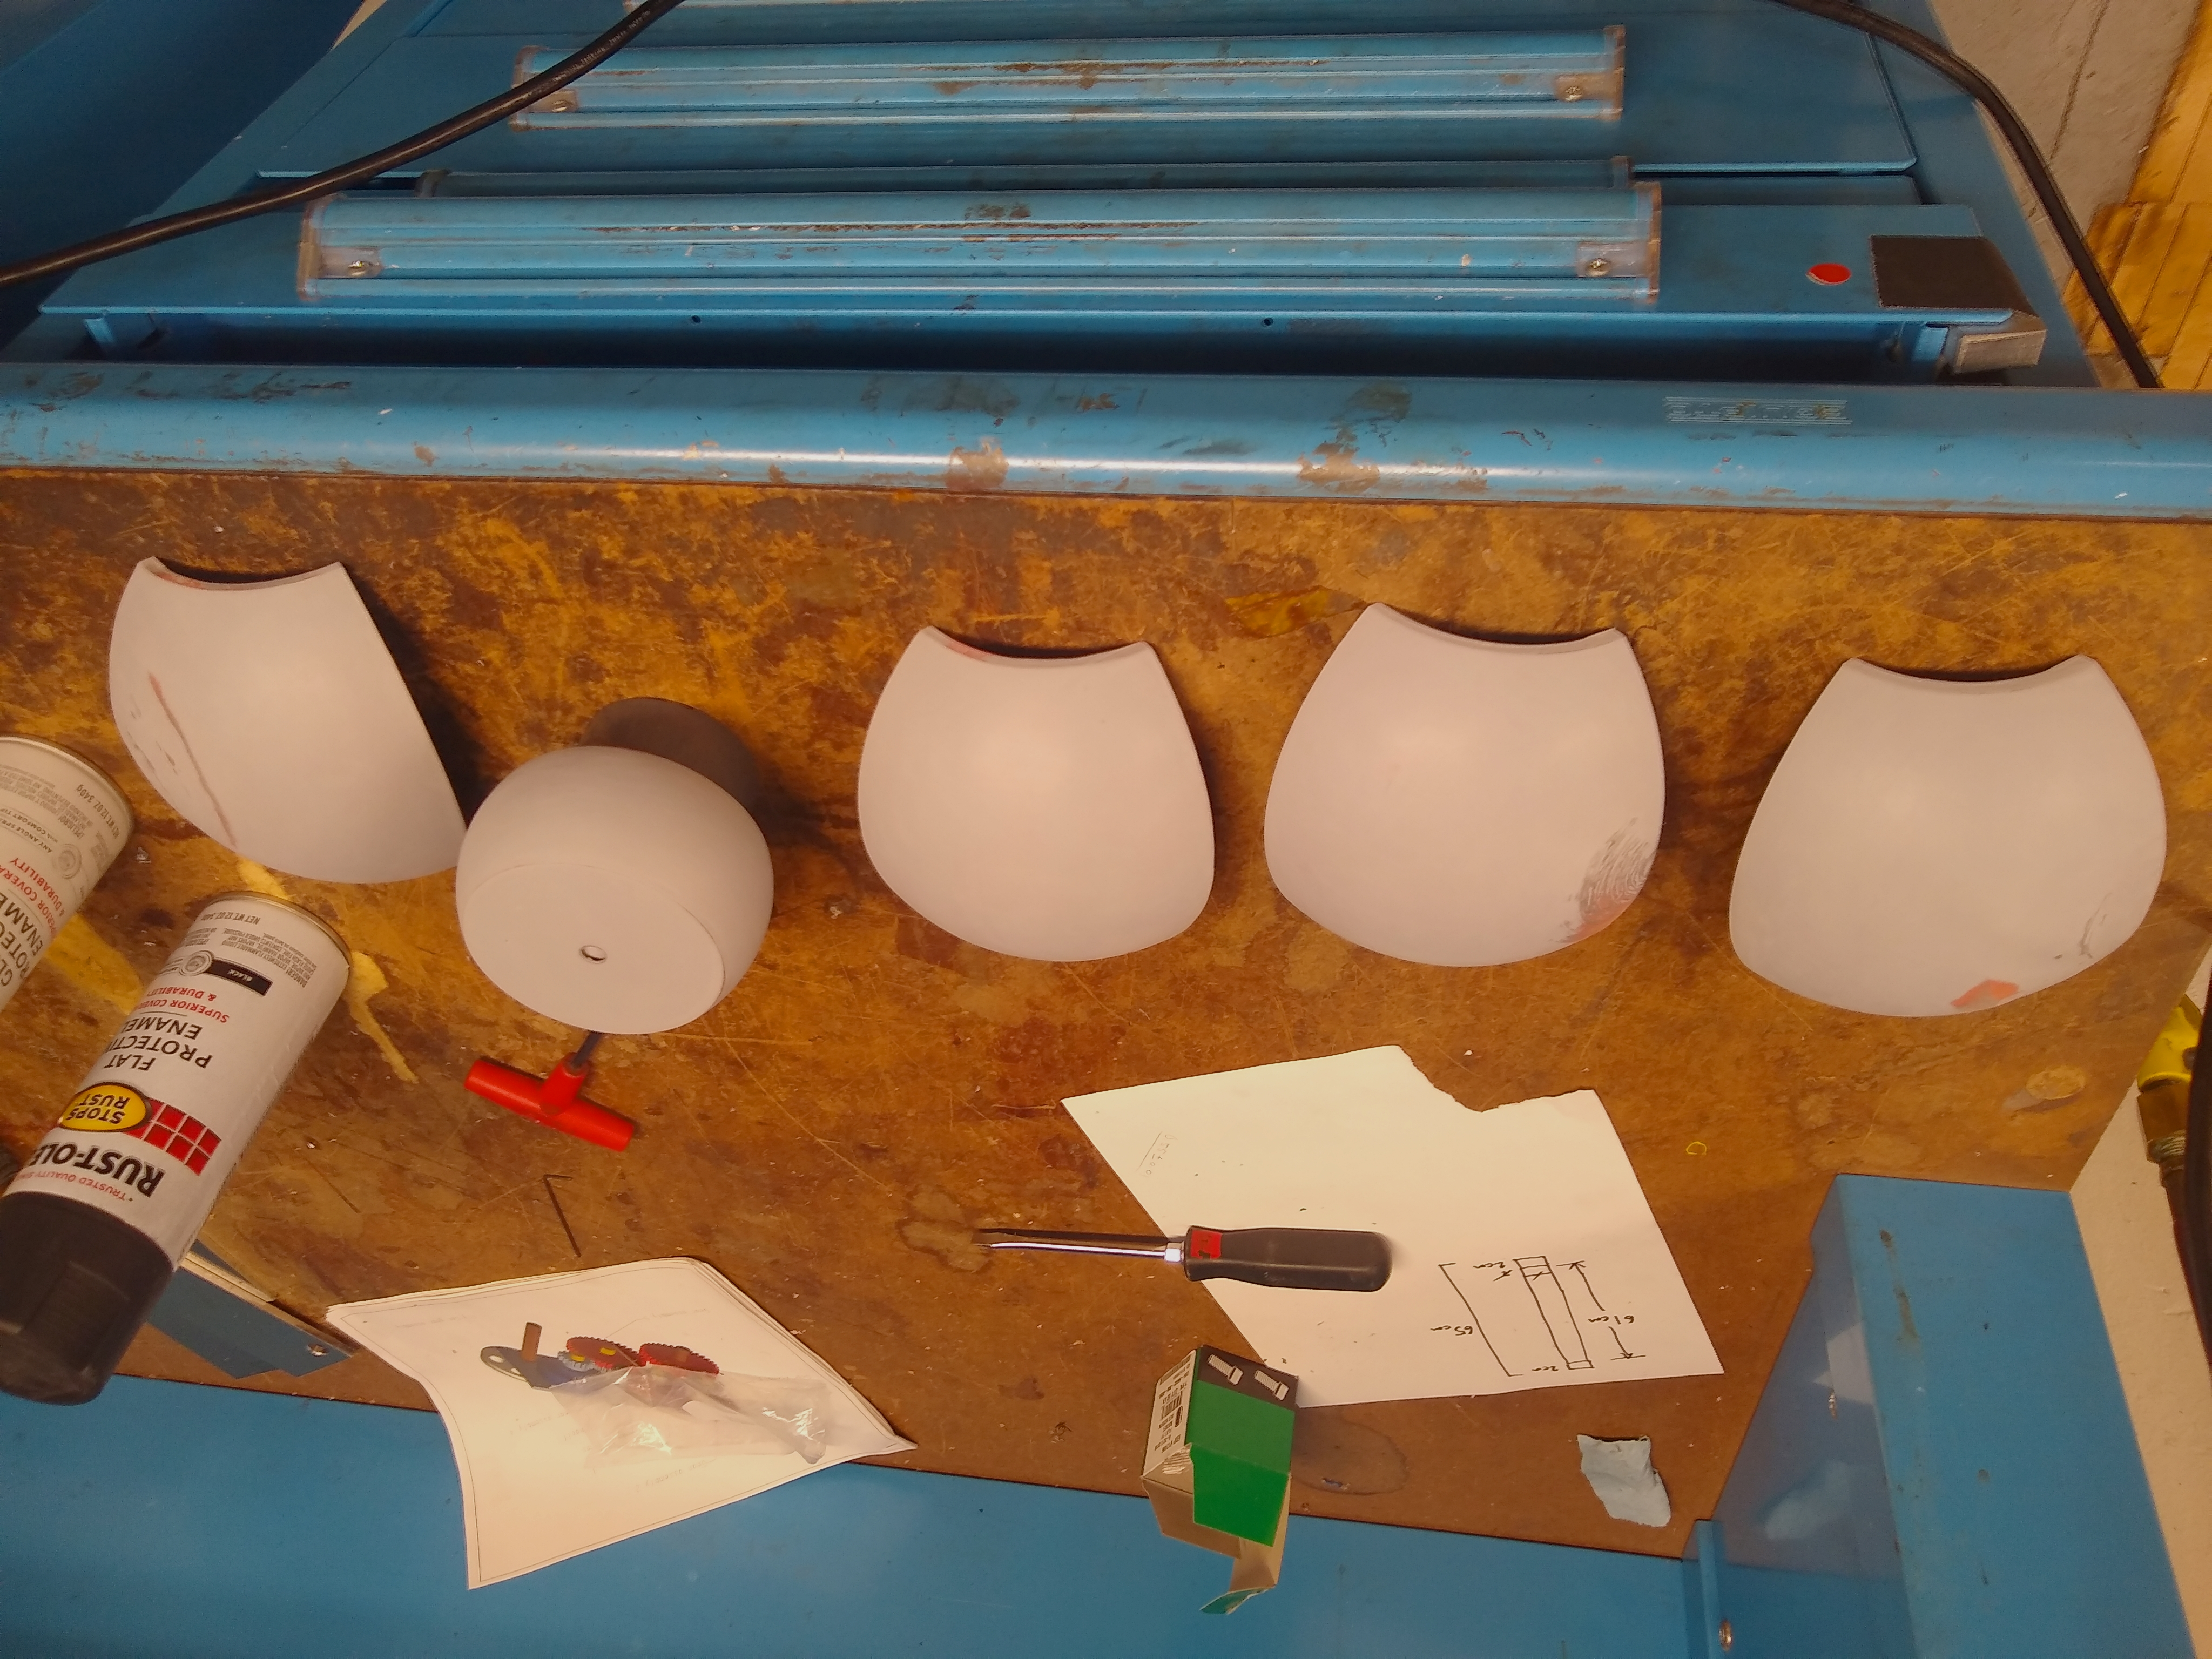
\includegraphics[width=\textwidth]{Thesis/ch3/manufact-2.jpg}}
    \caption{Filler Primer + sanding}
\end{subfigure}
\hfill
\begin{subfigure}{0.3\textwidth}
    \rotatebox{180}{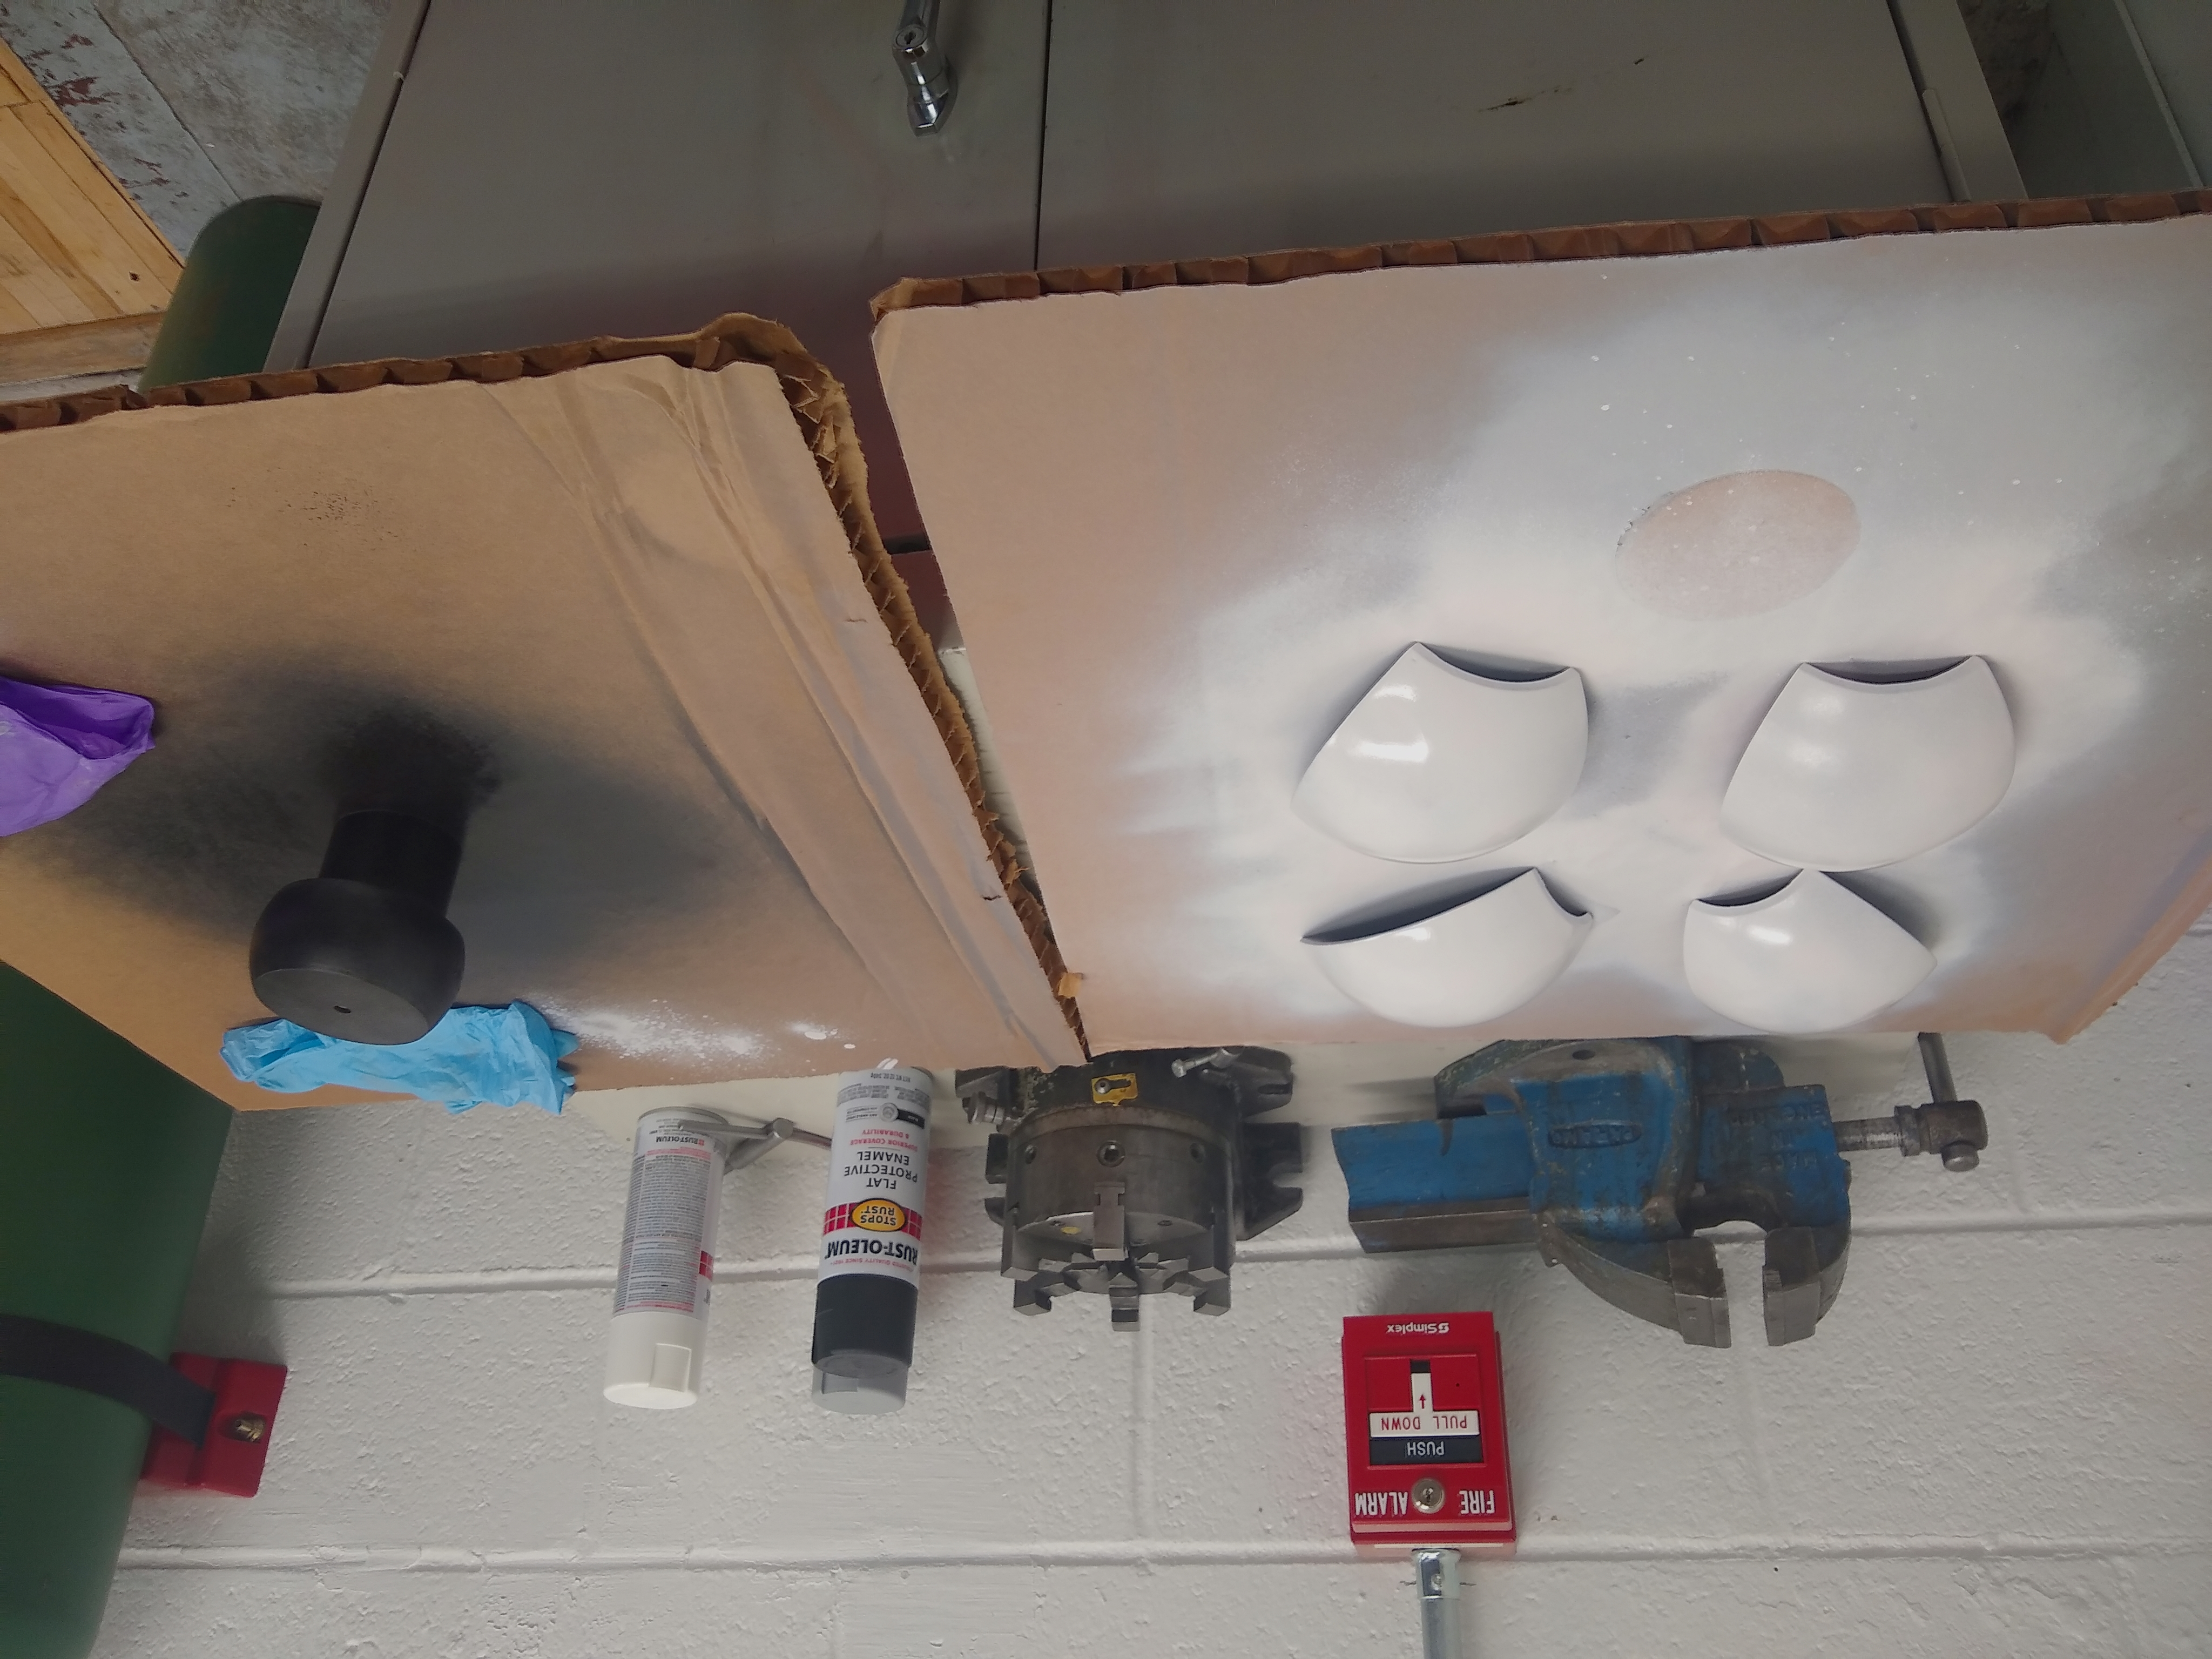
\includegraphics[width=\textwidth]{Thesis/ch3/manufact-3.jpg}}
    \caption{Spray Painting}
\end{subfigure}
\caption{Process of finishing parts}
\label{fig:manufact}
\end{figure}

\section{Mounting Components}
The head assembly was designed to accommodate the microcontroller, servos, and most of the wiring. This was done to keep a clean look to the robot. An image of the inside of the head can be seen in Figure \ref{fig:servo-shot}. The servos are mounted onto the mounting block with 8-32 screws. They are held in by heat set threaded inserts, which allows for metal threads to be added to a 3D printed part. This provides a strong metal screw hole, as opposed to tapping the plastic itself. To mount the camera, existing geometry of the product was leveraged. The camera enclosure is essentially a plastic box held together by four screws on the front face. By removing this front face, we can reuse these screw holes as mounting geometry, replacing the face of the camera enclosure with the front face of the eyeball. The eyeball part was designed such that the existing screws could mount the camera. The tolerances on such a small part were a challenge, so the previously mentioned iteration technique was used to get the part to fit properly. The Teensy daughter board was mounted with 5-40 screws, shown in Figure \ref{fig:teensy-shot}. These components are all mounted with screws, which was an an important consideration throughout the design process. This was to allow for the robot to be completely disassembled for troubleshooting and replacing broken parts.

\begin{figure}
    \centering
    \begin{subfigure}{0.4\linewidth}
        \rotatebox{270}{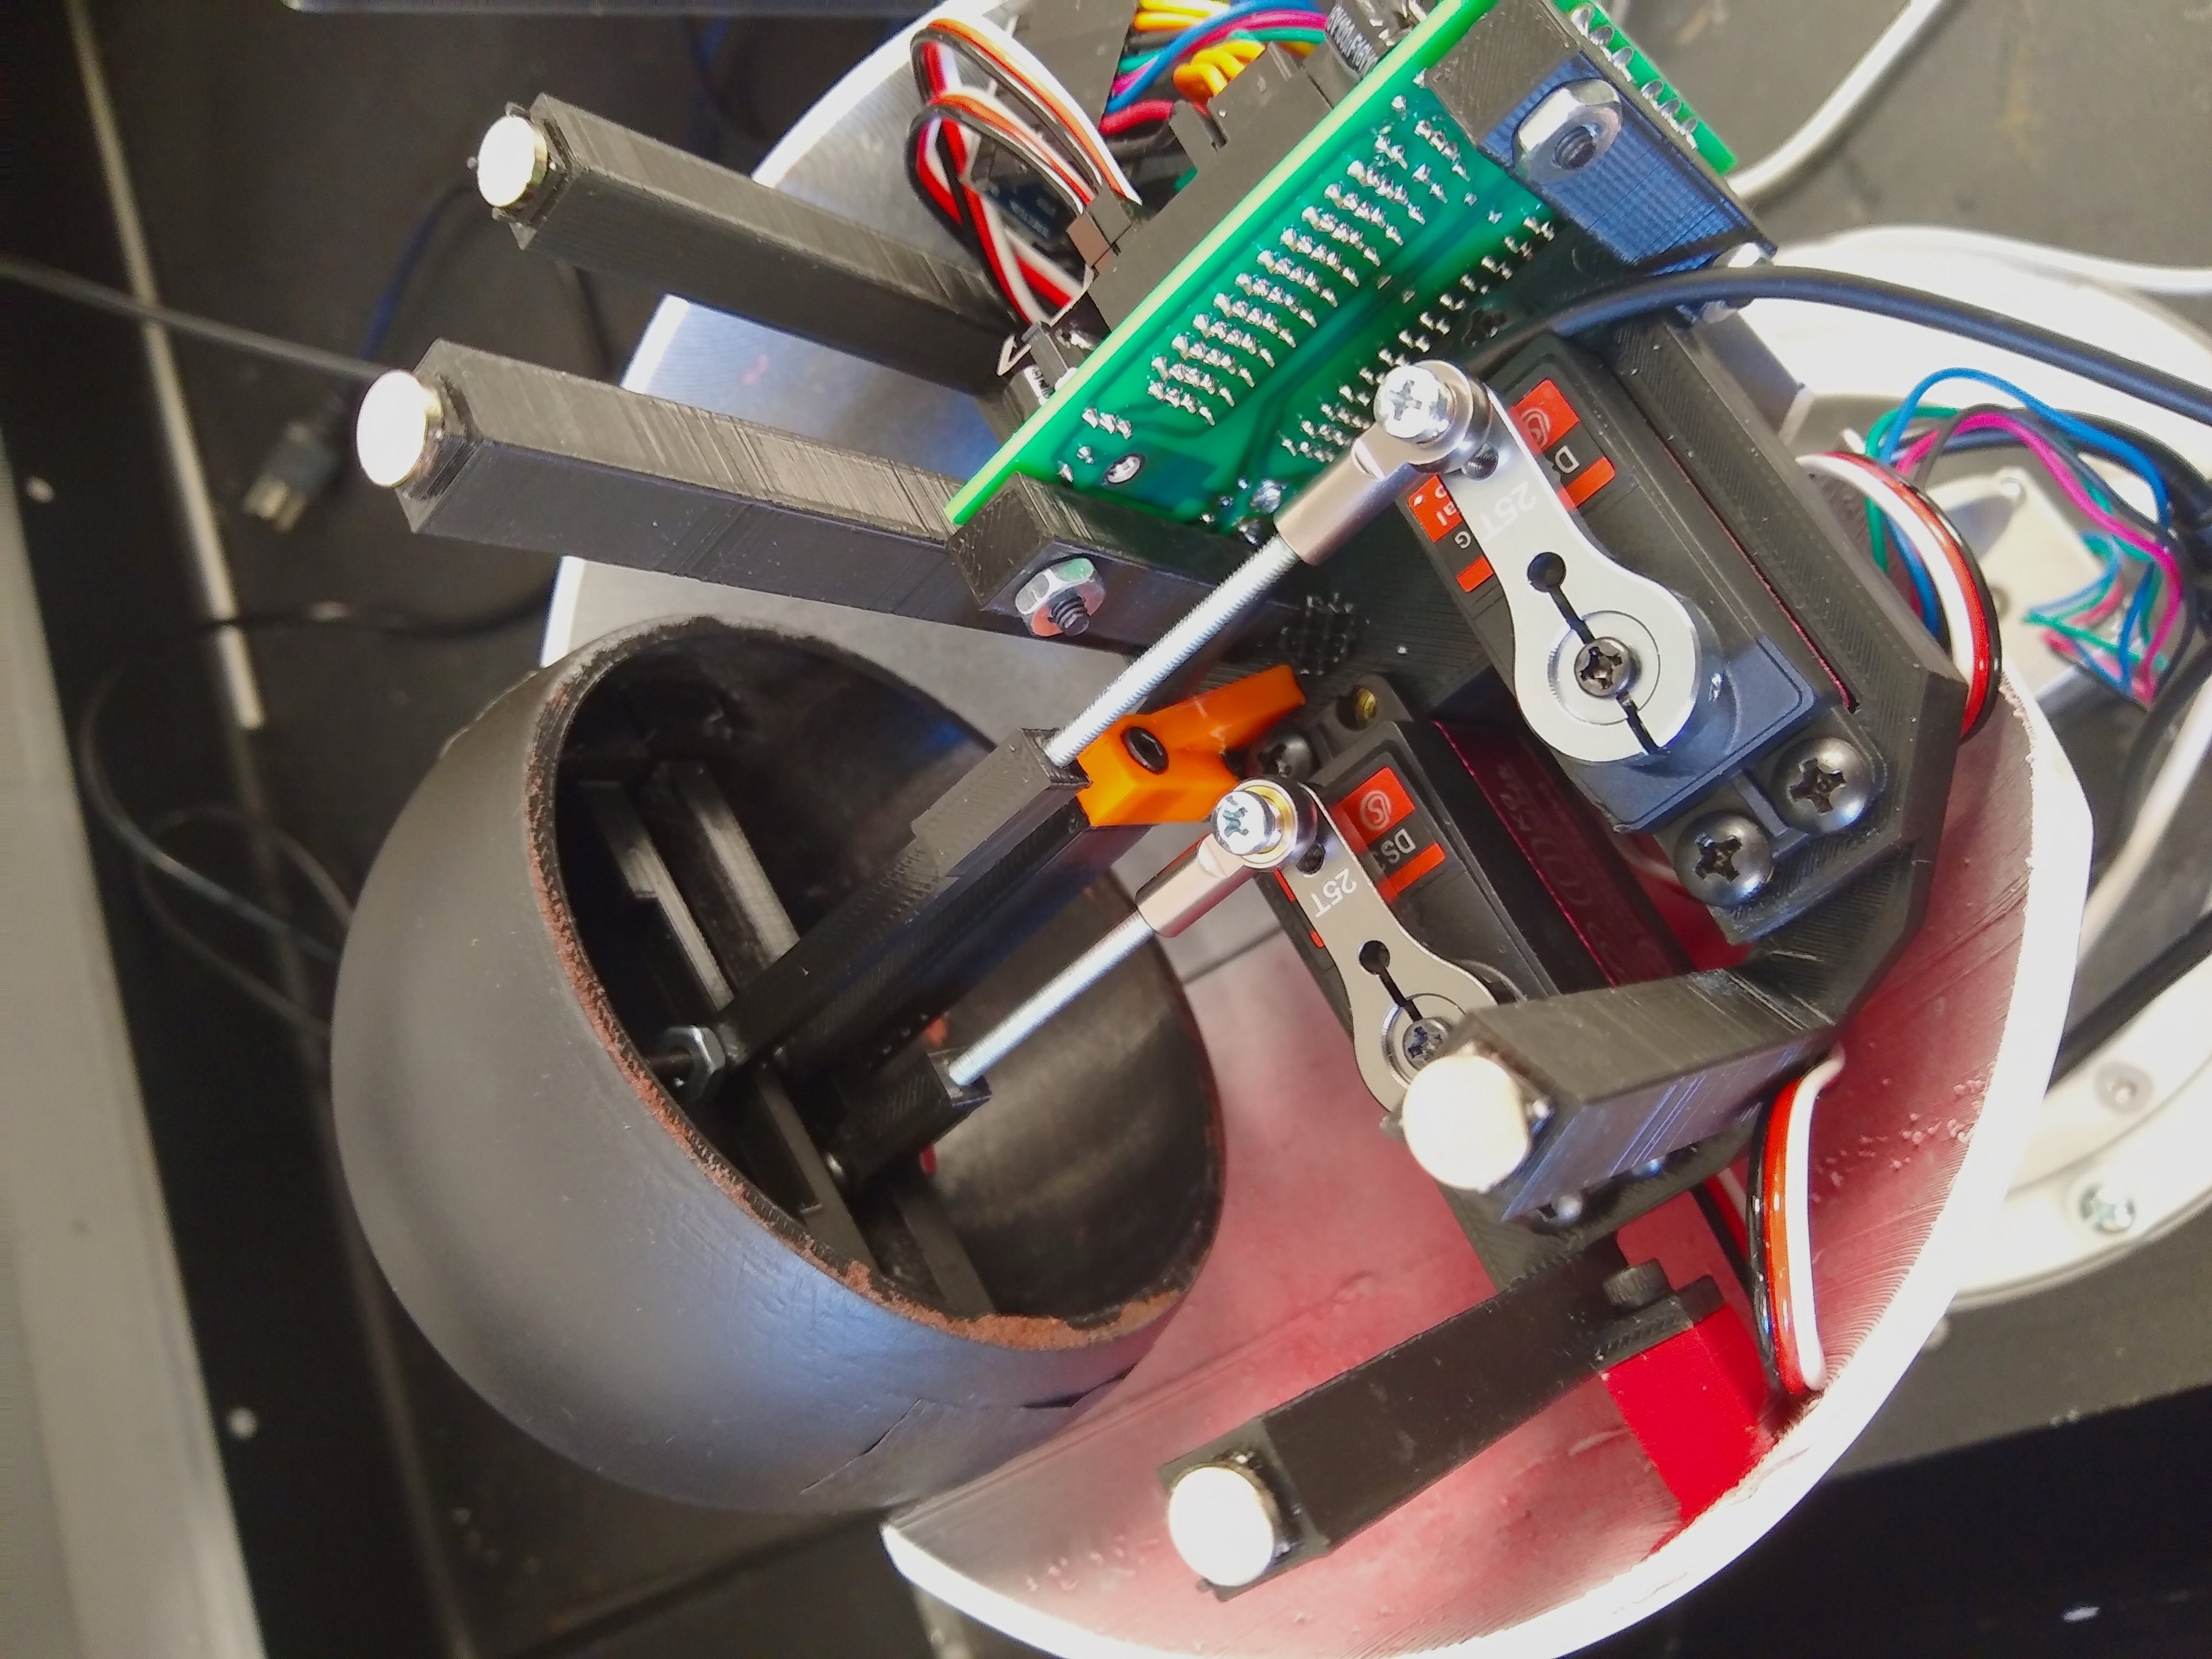
\includegraphics[width=\linewidth]{Thesis/appendix/photos/innerds-1.jpg}}
        \caption{}
        \label{fig:servo-shot}
    \end{subfigure}
    \begin{subfigure}{0.4\linewidth}
        \rotatebox{270}{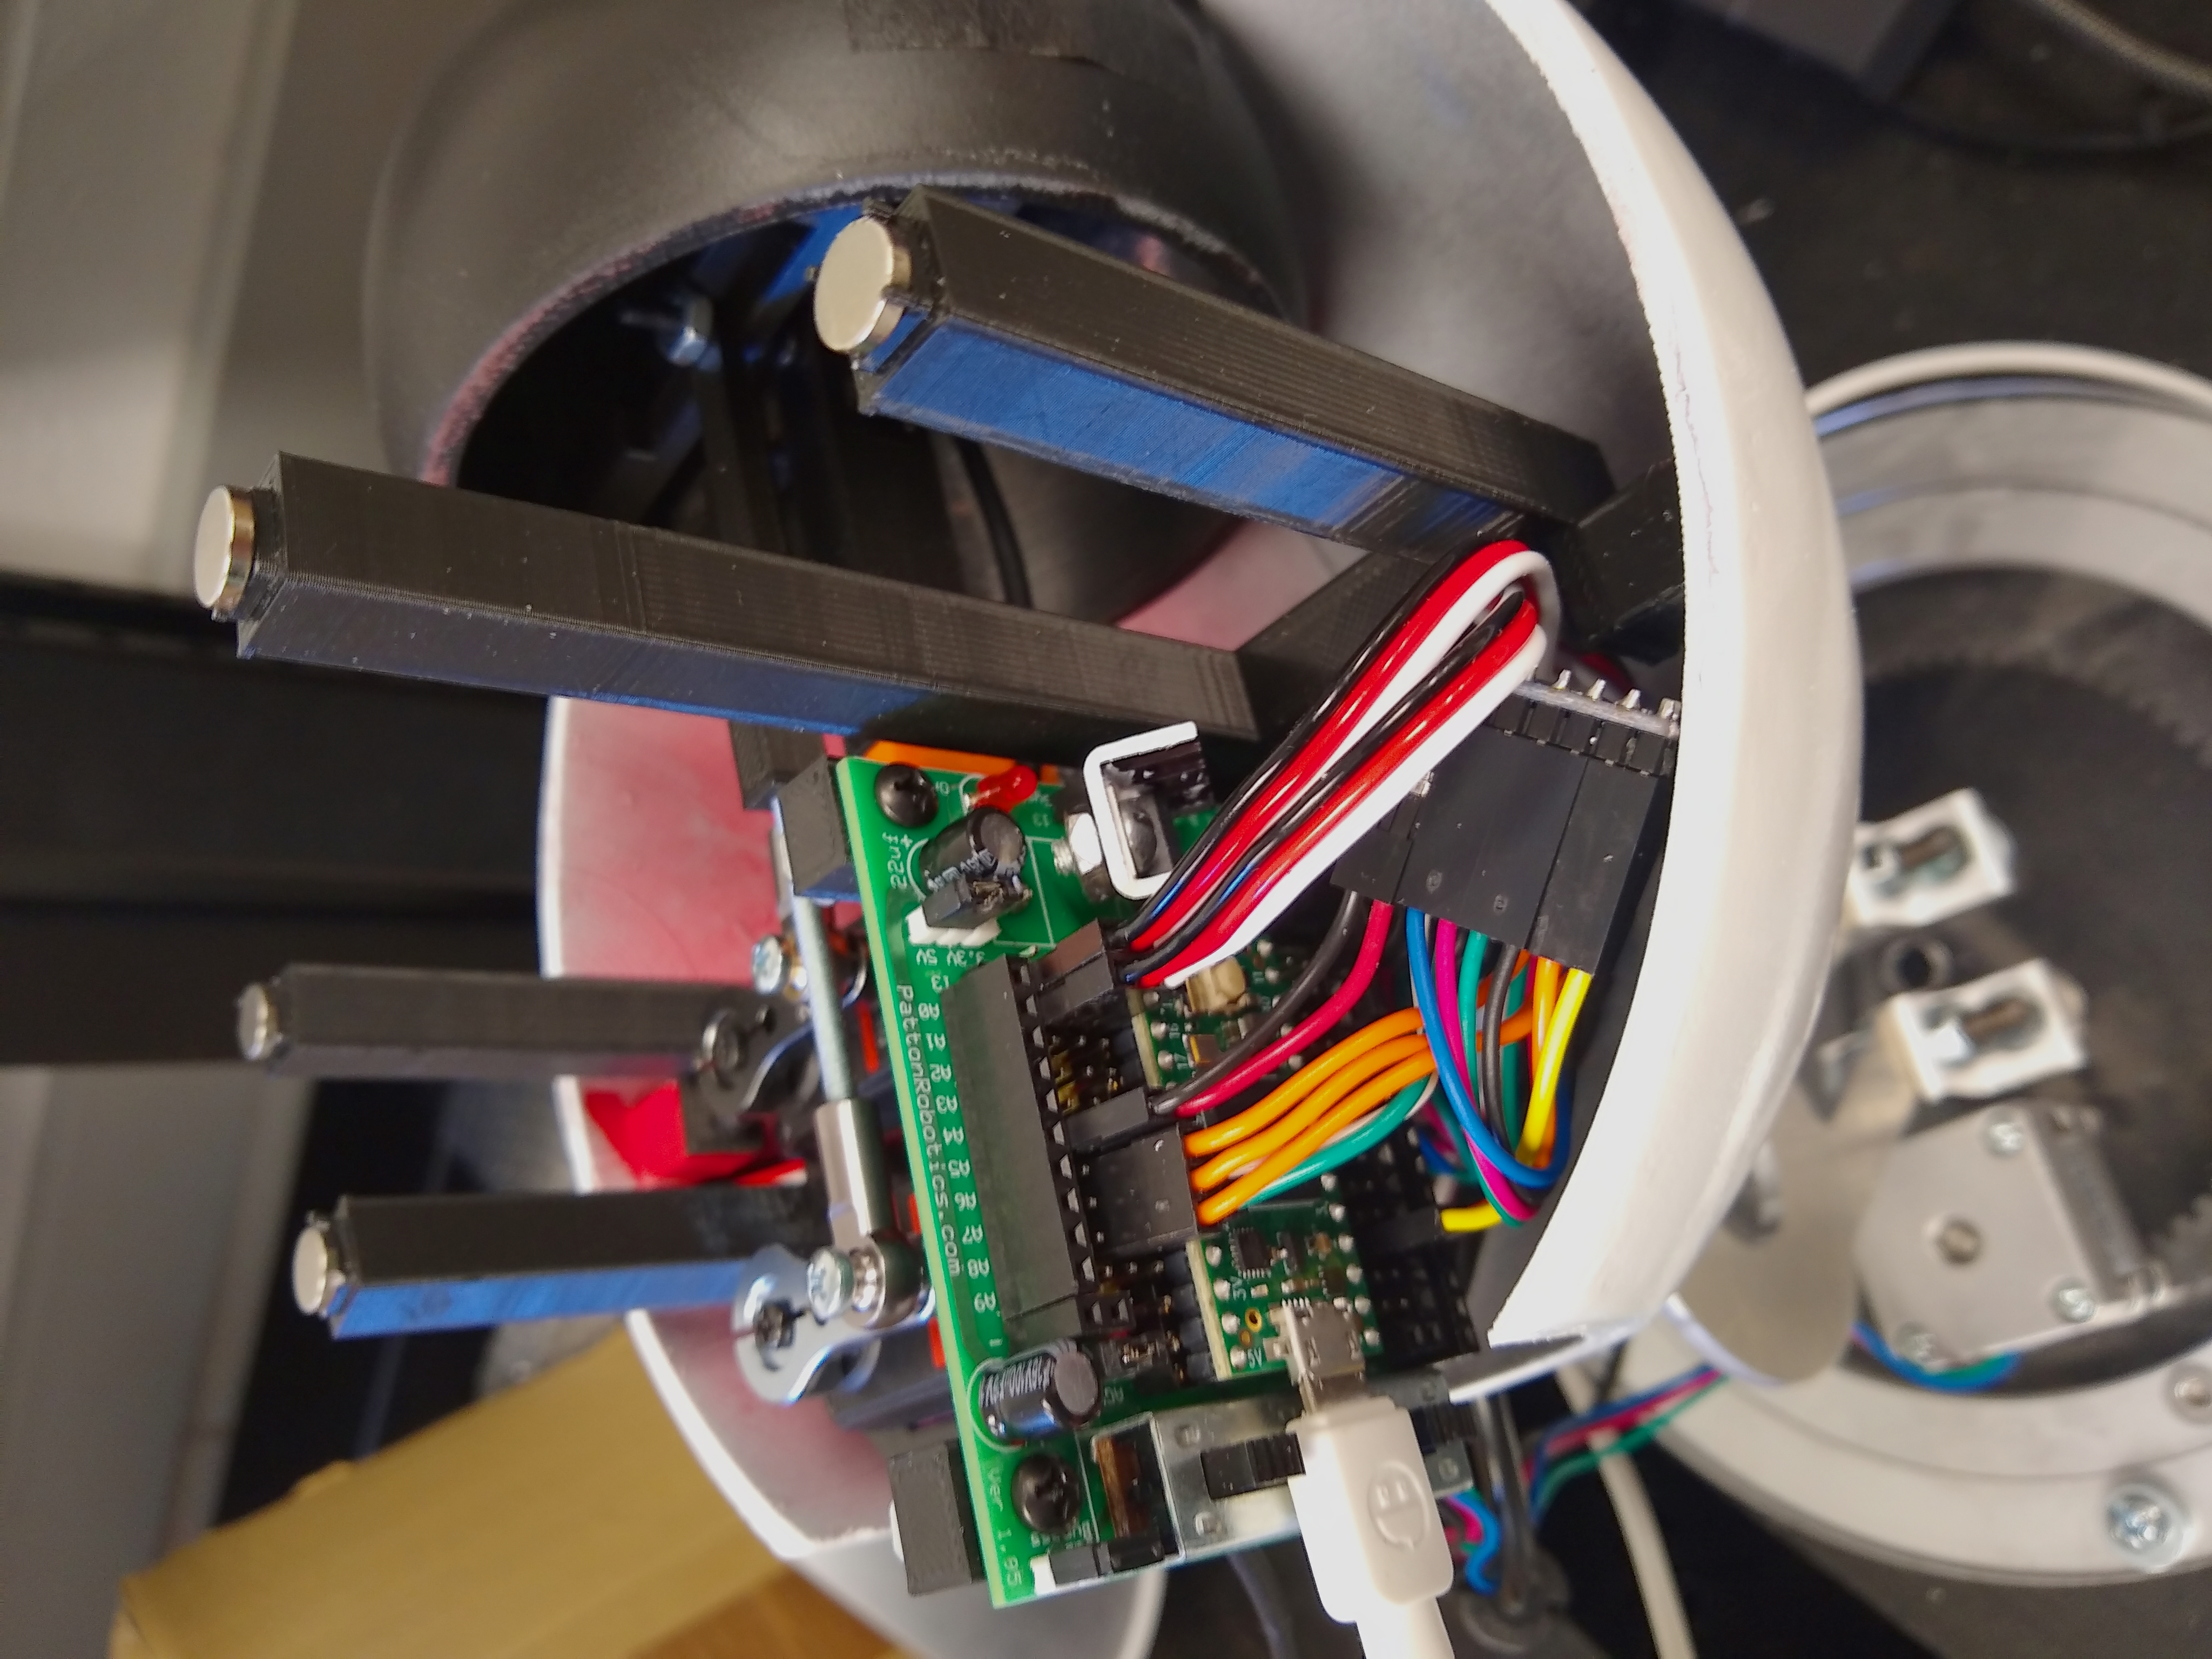
\includegraphics[width=\linewidth]{Thesis/appendix/photos/innerds-left.jpg}}
        \caption{}
        \label{fig:teensy-shot}
    \end{subfigure}
    \caption{View of the mounted components inside the head.}
    \label{fig:mounted}
\end{figure}

\section{Final Model}
The final model completed and assembled is shown in Figure \ref{fig:final_model}.
\begin{figure}[h!]
    \centering
    \includegraphics[width=0.6\linewidth]{Thesis/best-view.jpg}
    \caption{Photo of the final model.}
    \label{fig:final_model}
\end{figure}
\chapter{Electronics and Software}
One of the constraints set early on in this project was keeping the robot low budget. This meant that no proprietary algorithms or software could be used; everything had to be free and open source. Luckily, the internet has a wealth of different options that people have created and make open for others to use.
\section{Inspiration}
The first step of any electronics design is establishing the feasibility of the design goal. Various examples were found on the internet demonstrating similar projects and inspiration was drawn from them to incorporate into this project. For instance, in a video by the YouTube channel Core Electronics showcased face tracking camera using OpenCV and a Raspberry Pi, shown in Figure \ref{fig:core-electronics}. This seemed to be a good proof of concept and was important in establishing the feasibility of this project, especially in such a short time frame. The problem with this model is that it is nothing more than a proof of concept, rather than a full product. It has minimal electronic components and the mechanism is fairly simple. The pan servo moves the tilt servo completely, which accomplishes two degrees of freedom, but is simplistic and most importantly does not resemble a natural eye nor does it resemble the dynamics of my eye mechanism. Another thing to note is the speed and smoothness of the motion of the face tracking mechanism leaves much to be desired, which was an area focused on in this project.

\begin{figure}[h]
    \centering
    \includegraphics[width=0.3\linewidth]{Thesis/ch4/core-electronics.png}
    \caption{Pan and tilt mechanism used in the Core Electronics example.}
    \label{fig:core-electronics}
\end{figure}

\section{Components Selection}
\subsection{Microcontroller}
All components used in this project can be found in the Bill of Materials in Appendix \ref{ch:bom}. One important choice to note is the microcontroller, which is essentially the brain of the robot. The Teensy 4.0 was chosen for this for its low price but incredible speed. The Teensy can also be programmed in Arudino, which allows it to tap into the wealth of documentation and example code snippets online. To interface with the components it is possible to simply use a breadboard, but this project opted to leverage a dedicated robotics board to facilitate the process. This board, called PRT\_28 by Patton Robotics, provides numerous convenient features like a DC jack, voltage regulator, capacitors for despiking, and separate power rails for 12V and 5V. These are all components that could have been procured on their own, but for \$26 the board was the smarter choice given the time frame. A future version of the project would use a custom PCB that would allow for a large simplification of the circuitry. For instance, in hindsight much of the functionality of the Teensy is superfluous and can be accomplished with a much cheaper ATmega328P chip. Still, the Teensy accomplished what it was intended to, which was to serve as a way to control and synchronize the motion of the three motors in the robot.

\subsection{Actuators}
As stated in Section \ref{ch:design-iterations}, the motors chosen for the project were common, affordable parts. The servo model used in this design is the DS3218MG, with a control angle of $270^\circ$. 

Since the stepper motor is being geared up and the robot does not weigh much, the torque requirement on the stepper motor is not very large. As such, a smaller form factor was chosen to fit on the 8'' diameter base. The component chosen was a NEMA 14 stepper with 200 steps per rotation. With a control angle of 1.8 per step, these kinds of stepper motors are not known for their precision. However, this can be mitigated by gearing up the motor, which was explained previously, and choosing the right stepper motor driver.

To make the stepper motor spin, the electromagnetic coils in the motor have to be driven in the right order to spin the shaft. This can technically be done with the Teensy, but the smarter choice was to procure a daughter board with dedicated circuitry to efficiently drive the motor. This board, called the stepper driver, powers the stepper motor in accordance to signals from the Teensy. The one used in this project is a RepRap StepStick, running the A4988 chip \cite{bowyerStepStickRepRap2020}. This board communicates with the Teensy through two pins, denoted by the STEP and DIR (direction) pins. Every time the Teensy powers the STEP pin, the motor advances one step in the direction indicated by the state of the DIR pin. It is important to note that the motor is running at 12V, while the rest of the components use 5V. The stepper controller also serves the purpose of separating the two power lines and keeps the microcontroller safe from high voltage backflow. Another useful feature of the A4988 is microstepping, which allows the motor to move at fractions of a step. This enables much greater precision than the base 200 steps per revolution of the motor. For the greatest precision and smoothness of the movement, the lowest microstepping configuration was selected at 1/16 step, now giving the motor 3200 steps per revolution. Combined with the 1:6 gear ratio, this allows the stepper motor to rotate the robot with a resolution of $200\times16\times6=19200$ steps per revolution, or $0.01875^\circ$ per step.

\subsection{Miscellaneous}
A 12V 5A AC adapter of was used to deliver power to the circuit. The 12V of the jack powers the stepper motor directly and passes through a voltage regulator to power the rest of the 5V circuitry.

Additional components include a speaker and microphone which were incorporated into the design for a nominal user to have a natural conversation with the robot listening and responding. The current functionality is limited to playing sound files from a Python script, but the main purpose of including these components was to future proof the design for features that are planned to be included later down the line.

\section{Circuit Diagrams}
The circuit diagram used to wire up the components can be seen in Figure \ref{fig:circuit_diagram}. Note that the only components that had to be wired up were the Teensy microcontroller, the two servos, the stepper motor and its associated motor controller board. The other components, such as the camera, microphone, speaker, and the Teensy serial data cable all used a plain USB 2.0 connector, so they simply needed to be plugged into a USB hub and connected to the computer. One thing to note is that the 5V power line of the Teensy USB cable is cut. This isolates the Teensy power from the laptop and allows the laptop to communicate with the microcontroller over the two data lines without the potential of any backflow voltage that could damage the laptop. These USB cables come out of the back of the robot's head, pictured in Figure \ref{fig:back-wires}.

\begin{figure}[h]
    \centering
    \includegraphics[width=0.8\linewidth]{Thesis/ch4/theses-schematic-2.pdf}
    \caption{Electrical schematic of the circuit. Generated in Autodesk EAGLE.}
    \label{fig:circuit_diagram}
\end{figure}

\begin{figure}[h]
    \centering
    \includegraphics[width=0.4\linewidth]{Thesis/ch4/back-wires.jpg}
    \caption{A photo showing the wires coming out of the back of the head.}
    \label{fig:back-wires}
\end{figure}
\section{Software and Programming}
The algorithm for following the eyeball needed to be simple but also fast. One measure taken was avoiding the practice of blocking, which is when the processor waits for one action to finish before beginning the next. This would essentially freeze the Arduino when any motor is running and rather than all the motors moving at once, causing them to move one after the other. Instead, the code utilized software libraries that used non-blocking code to drive the actuators, which enabled all the components to move at the same time. This helps with smoothing out the motion of the system and keeping the robot more appealing to interact with. 

\subsection{Software Libraries Used}
\begin{itemize}
    \item Python
    \begin{itemize}
       \item OpenCV 2 \cite{OpencvOpencv2023}
        \item face\_recognition \cite{geitgeyFaceRecognition2023a}
        \item pySerialTransfer \cite{powerbroker2PySerialTransfer2023}
    \end{itemize}
    \item Arduino
    \begin{itemize}
        \item SerialTransfer \cite{pb2SerialTransfer2023}
        \item ServoEasing \cite{arminServoEasing2023}
        \item AccelStepper \cite{AccelStepperAccelStepperLibrary}
    \end{itemize}
\end{itemize}

\subsection{Control Loop}
Figure \ref{fig:control_loop} shows the control loop for the program. The control is discrete rather than analog, since the microcontroller runs in discrete time steps. The algorithm is as follows: First, the camera on the computer turns on and receives an image. An example of the image output from the camera is shown in Figure \ref{fig:face-example}. Then, the Python facial recognition library is used to find the center of the bounding box drawn around the face in the image and calculates the distance from that point to the center of the image. This distance is then scaled by a constant and sent as a move command to the motors. One effect of this approach is that larger move commands are sent to the motor as the face is farther from the center of the screen. This ensures that the camera will reach the face in fewer moves than a constant stepping distance. As the face gets closer to the center of the image, the motor commands are smaller, giving the system the ability to perform micro adjustments to center the camera properly.

A deadzone is used to decide whether or not to command the motors, since it is practically impossible that the face will be at the very center pixel of the image. The deadzone chosen for this was the middle 6\% of the width and height of the image. This seemed to provide a good balance between allowing for imperfect alignments while still producing a convincing face-tracking result to the user.

The servo and stepper motors in turn move the camera, which then captures a new image and the cycle repeats. It is important to note that the move commands are relative to the actuator's current position, so the Python code does not actually know what position the motors are at. All it sees is the camera footage and sends commands to the Teensy. Once the Teensy is ready to receive a command, it picks the most recent one out of the stack and executes it. Of course, there are some hard coded limits in the code to make sure the actuators do not exceed the maximum designed range of motion, which would cause the machine to tear itself apart, which is discussed in more detail in Section \ref{ch:safety}.

To decide when to use the stepper vs the X-servo to correct the x-position of the camera image, the X-servo was set to run 70\% of the distance total distance and the stepper was set to run 30\%, so that when they are run at the same time they center the camera correctly.

The control loop models a proportional controller, since the control output linearly scales with the measured input. The full Python and Arduino code can be found in Appendices \ref{ch:python-code} and \ref{ch:arduino-code}, respectively. Lots of the skeleton code for this algorithm was based on examples provided by face\_recognition, pySerialTransfer, and SerialTransfer.

\begin{figure}[h]
    \centering
    \includegraphics[width=0.9\linewidth]{Thesis/ch4/Microcontroller (3).pdf}
    \caption{Control Loop for the face tracking algorithm.}
    \label{fig:control_loop}
\end{figure}

\begin{figure}
    \centering
    \includegraphics[width=0.5\linewidth]{Thesis/ch4/face-example.png}
    \caption{Example of what is displayed on the screen for facial recognition.}
    \label{fig:face-example}
\end{figure}

\section{Actuator Range of Motion}
\label{ch:safety}
To command the servos to move to a set position, the microcontroller sends it a PWM pulse in the range of 500-2500 ms, where 1500 ms is the middle position of the motor's range of motion. The eye mechanism does not need the full 270 degrees range of motion of the servos, in fact if the servos rotate that far it will tear the mechanism apart, which happened multiple times by accident. For this reason the millisecond ranges allowed to be sent to the servo were trimmed. 

The mechanism was designed so that the motors would hold the eye in a neutral position looking straight ahead when the servos are in their middle 1500 ms position. However, due to assembly imperfections this was not actually the case, so the motors had to be calibrated to find the servo position that would produce the desired neutral position of the eye. As such, after some experimentation these limits were empirically set to 1200-1670 ms for the Y-servo and 1320-1680 ms for the X-servo. Translating this into real world measurements, this means that the arm of the Y-Servo and X-Servo can sweep through an angle of $63.45^\circ$ and $48.6^\circ$, respectively. The stepper motor limits were determined such that the beyond $180^\circ$ in either direction to protect the cables from getting wrapped up. Since a full rotation of the robot would be 19200 steps, the limits on the motor were set to 9560 steps in either direction.

A confusing detail to note is that in the software the ends of the servo rotation are called 0 and 180, but these are just arbitrary variables. The true angular displacement of the robot is scaled according to the inputted ``angle'' and the microsecond range previously mentioned. For instance, a servo command of 90 to both motors resets the mechanism and returns it to the neutral looking ahead state. For simplicity, from this point forwards the servo angles will be referred to by their software variables rather than their real world counterparts.

\section{Integration}
Integrating these different components together was a significant challenge. Most notably, the facial recognition library is written in Python and is too computationally intensive to be run on a microcontroller, so the code has to be run on a PC instead. The PC then has to communicate with the Teensy through the Python script to tell the microcontroller how it should move the actuators. Fortunately, the serial data system is designed for this purpose.

Serial data allows for digital data to be sent through electrical signals in a cable to the microcontroller. This data can then be interpreted as a integer, character, or other any data type. This works both ways as well, so the microcontroller can also send values to the PC. This is a relatively trivial task if only one value is being sent to the Teensy, since Arduino has built in serial libraries for this purpose. For instance, I can type in the letter b on my computer and the PC sends it over the USB cable, then the microcontroller can recognize that data and do something with it, like printing out the value or moving a servo according to an inputted number. \cite{ansh2919SerialCommunicationPython2021}\cite{detheFaceTrackingOpenCV2019}. However, the challenge is controlling multiple actuators at once. The stock Arduino library uses blocking code, so this would slow down the system tremendously. Also, the microcontroller needs some way to identify which commands to send to which motor. This can be done with the base Arduino library \cite{robin2SerialInputBasics2016}, but a more complete solution was to use pySerialTransfer.

The pySerialTransfer library takes advantage of the C data structure \emph{struct}, which allows for packaging multiple variables into a single data structure. This struct is composed of the two servo move commands and the stepper move command. This allows us to separate the move commands into distinct variables that can be read and used by the microcontroller. The struct is first filled with values by the Python script based on the previously mentioned methodology, then the Python script fills a buffer with the struct. Once it finishes putting all three values in the buffer, it sends it off to the Teensy with serial data. The library pySerialTransfer interprets this serial data and fills in the corresponding struct in the Arduino script with the appropriate move commands. Then, the Teensy can use these values to actuate the motors accordingly. The full setup, including the robot and laptop, can be seen in Figure \ref{fig:complete-setup}.

\begin{figure}[h]
    \centering
    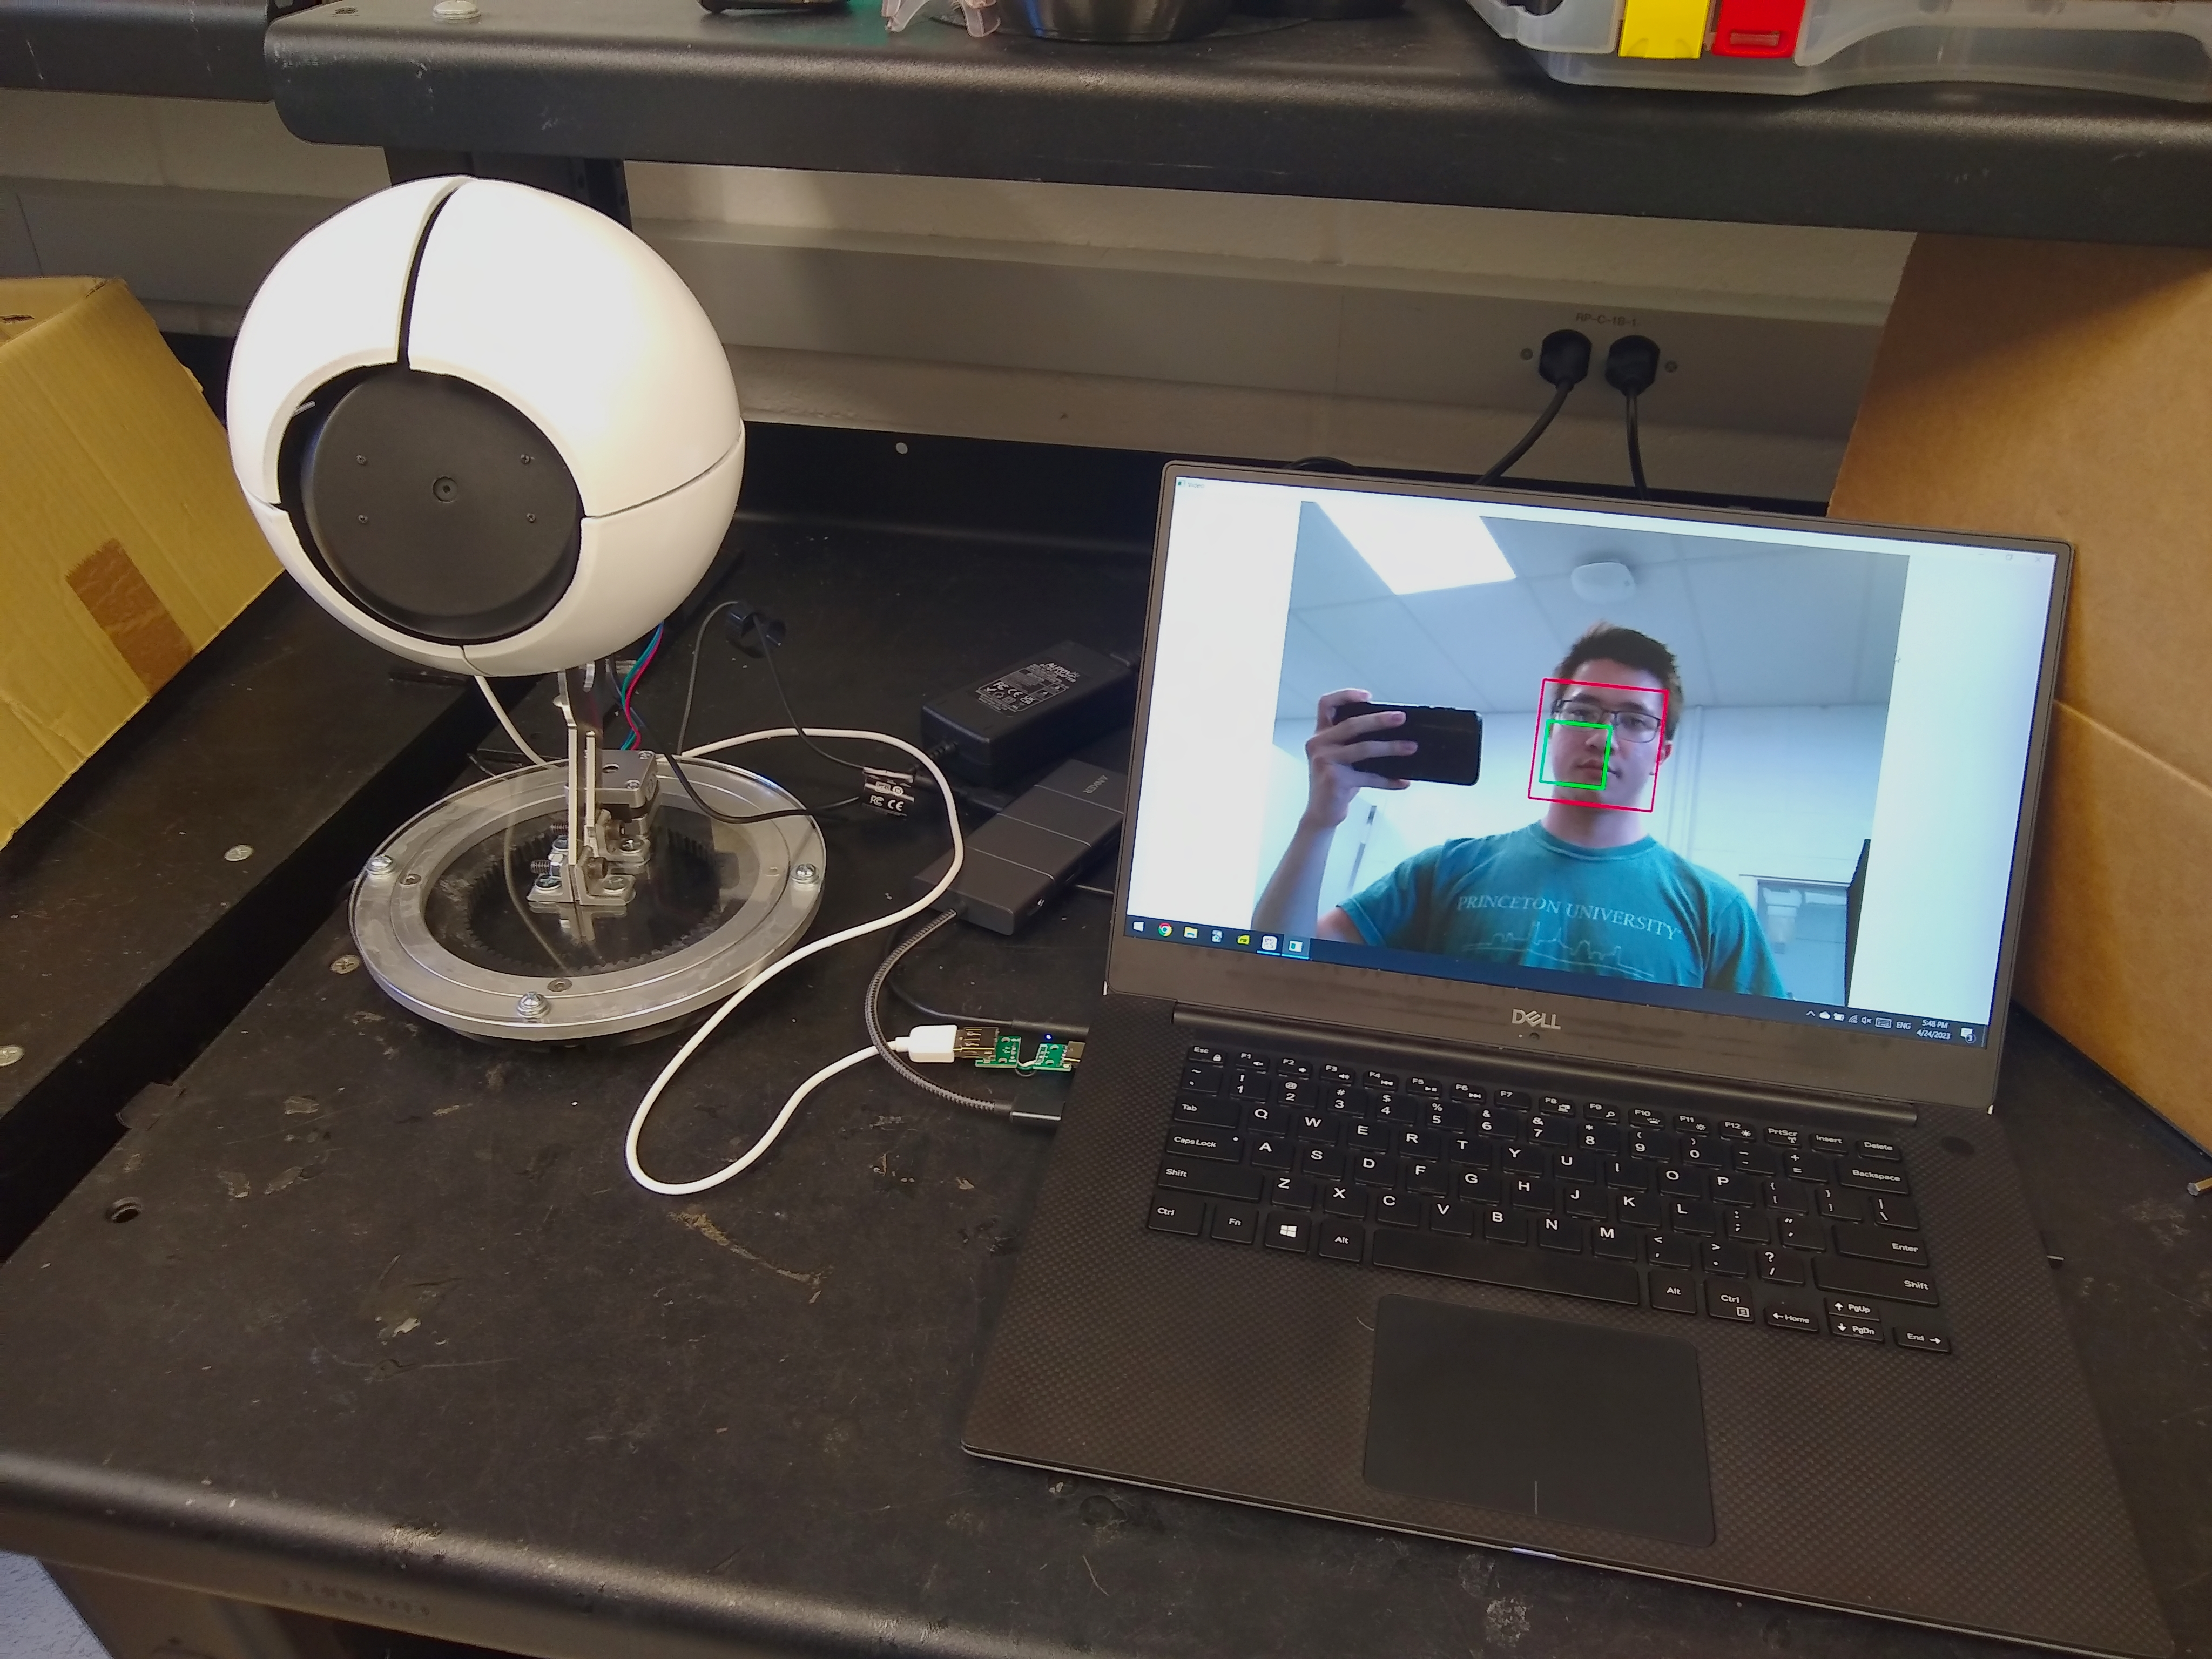
\includegraphics[width=0.5\linewidth]{Thesis/ch4/full-setup.jpg}
    \caption{Photo of the entire setup.}
    \label{fig:complete-setup}
\end{figure}
\chapter{Results}
\section{Dynamics}
Early versions of the robot used arbitrarily chosen scaling to approximately get the motions right, but a more numerical concert approach based on the dynamics of the system was desired to tune the parameters. The dynamics of the system start at the servo inputting an angle, which then transfers through numerous pin linkages before finally being outputted by the camera seen by the computer. As such, a test was set up to find the relationship between the servo angular displacement and the resulting planar image movement. The test was done by making a custom Python script that only controlled a single axis at a time. The script would record the center of the recognized face, while the user looked at it keeping their face as still as possible, then advance the angle of the servo by 3 degrees, then repeat. This loop ran until the face had moved out of frame of the camera and the software could not see a face anymore. The stepper motor was tested the same way, just was instead told to advance 100 steps every loop. The tests were done over three trials and averaged. The results of the data are plotted in a scatter plot form in Figure \ref{fig:scatter}.

\begin{figure}[h]
    \centering
    \begin{subfigure}{0.475\linewidth}
    \includegraphics[width=\linewidth]{Thesis/ch5/Face X Coordinate vs X-Servo Angle Displacement.pdf}
    \end{subfigure}
    \begin{subfigure}{0.475\linewidth}
    \includegraphics[width=\linewidth]{Thesis/ch5/Face Y Coordinate vs Y-Servo Angle Displacement.pdf}
    \end{subfigure}
    \begin{subfigure}{0.475\linewidth}
    \includegraphics[width=\linewidth]{Thesis/ch5/Face X Coordinate vs Stepper Displacement.pdf}
    \end{subfigure}
    \caption{Scatter Plots of Resulting Face Location}
    \label{fig:scatter}
\end{figure}

A line of best fit was calculated using the data collected in the tests. The slope of the line of best fit was found for each trial and then averaged for a final result, shown in Table \ref{tbl:averages}. It was found that for the Y-Servo, for every degree the servo arm moves, the face in the image moves by 7.98 pixels. The results for the X-Servo were similar, with a slope of 7.28. For every step of the stepper motor, it was found that the image moves 0.25 of a pixel. This makes sense since a full revolution of the robot would require 19200 steps, so step commands sent to the motor should be much higher than the servo command to move the same angular displacement. The results of these tests were then used to inform the parameter values of the motor commands in the Python script. The values are used as the scaling factor that converts the distances in the image to the servo movement commands, as seen in Appendix \ref{ch:python-code}. 

\begin{table}[h]
    \centering
    \caption{Average slope of regression line for 3 trials.}
    \label{tbl:averages}

    \begin{tabular}{c|c|c|c|c}
         & Trial 1 & Trial 2 & Trial 3 & Average\\
        \hline
        Y-Servo & -8.133 & -7.972 & -7.835 & -7.980\\
        X-Servo & -7.302 & -7.253 & -7.280 & -7.278\\
        Stepper Motor & -0.242 & -0.243 & -0.248 & -0.244\\
    \end{tabular}
\end{table}

\section{Speed and Acceleration}
From the datasheet of the servo, the maximum rotational speed of the servo is 0.16 sec/$60^\circ$, which corresponds to 6.54 rad/s. Early versions of the algorithm drove the motors at their maximum speed, but this produced a jarring and jerky movement. Moreover, rapid movements of the camera cause the image to blur and impede the facial recognition accuray. For this reason, the speed of the servos were limited in the software. As such, the ServoEasing and AccelStepper libraries were used in Arduino to add smooth acceleration and deceleration to the eye movements to make them more natural and inviting. This set a software limit to the speed and acceleration of the robot, The speed was set to 80 degrees/sec in software, which corresponds in the real world to 0.98 rad/s. The X servo was also set to this value, but since the microseconds limits were different this corresponds to 0.75 rad/s. There was no acceleration set for the servos to give them a faster response time. In fact, servo motors have a slight wind up naturally as the motor overcomes its stationary inertia, which another reason why software acceleration was deemed unnecessary.

Similar reasoning applied to the stepper motor. The torque curve of the motor provided by the manufacturer indicates that the maximum speed of the motor is around 4000 half steps per second, which corresponds to a rotational speed of 1005 rad/s. Not only is this much too fast for normal operation, but also the torque of a stepper motor drops off at higher speeds, therefore the max speed was set to 3000 step/s in the software, which corresponds to 15.7 rad/s after the 1:6 gear ratio. The maximum acceleration of the stepper motor set to 1000 steps/s$^2$ to give it an ease-in ease-out animation. This corresponds to a real-world rotational acceleration of 5.24 rad/s$^2$.

\section{Time}
\label{ch:time}
With these parameters set, the actual output of the robot had to be measured to validate its performance. For this purpose, the time required for the robot to cycle through the full field of vision was recorded. The results of this test are shown in Table \ref{full-move-times}. This was done with a custom script that swept the two stepper motors through their full range of motion and another script that did the same for the stepper motor. Since the eye servos are synchronized in the software such that they will always reach their end points at the same time, both servos were timed simultaneously producing a single measurement, as shown in Table \ref{full-move-times}. The average time for the eye mechanism to sweep from one side to the other was 4.248 seconds. The average time for the motor to sweep from $-180^\circ$ to $+180^\circ$ was 5.936 seconds. Ignoring acceleration,this corresponds to an average rotational velocity of 0.26 rad/s for the Y-Servo and 0.20 rad/s for the X-Servo, which is well within the bounds set in the software. The stepper motor is moving at an average velocity of 1.06 rad/s, which also falls within the maximum value set in the software. This ensures the safety of the user as the robot will not behave unpredictably and move faster than the software tells it to, even when it is making movements over the complete range of motion.

\begin{table}[h]
    \centering
    \begin{tabular}{c|c|c}
    Trial & Servos & Stepper \\
    \hline
    1&4.28&5.81 \\
    2&4.57&6.06\\
    3&4.15&6.17\\
    4&4.13&5.75\\
    5&4.11&5.89\\
    \hline
    Average&4.248&5.936
    \end{tabular}
     \caption{Measurements on the amount of time required for the motors go through a full move.}
     \label{full-move-times}
\end{table}


\section{Field of View}
\label{ch:fov}
According to B\&H Photo Video, the camera has a base field of view of 78 degrees \cite{b&hphotovideoLogitechC615Webcam}. The camera output is 16:9 ratio, but unfortunately the Python library crops the image to 4:3 for the facial recognition to work, so a test was done to find the resulting field of view after all the software distortions. The facial recognition software was set to run in a loop. I then moved myself to the very edge of the frame, where if I moved even slightly in one direction my face would stop being registered. Then, a marker was placed on the floor directly below me. This was done three times in both directions for a total of 6 measurements. Then, a line was drawn through these points and insersected at a point. The angle between the two lines is the measured field of view of the camera. The field of view was found to be around 60 degrees, shown in Figure \ref{fig:basic-fov}. 

However, with the actuation of the motors, it can be said that this affords the device a much better effective field of view. Since the eye can rotate the camera left and right, this allows the camera to see more of its environment. As such, a similar test was run with the camera panned to its maximum angle left and right, measurements were taken, and the angle between the lines was measured. With the range of motion the effective field of view was measured to be $130^\circ$. Figure \ref{fig:actuated} shows this in the green portion. The stepper motor also increases this field of vision. Since it can move through a full $360^\circ$ range of motion, this increases the effective field of view of the robot to $360^\circ$. This can be seen in the diagram as the blue circle.

\begin{figure}
    \centering
    \begin{subfigure}{0.4\linewidth}
        \includegraphics[width=\linewidth]{Thesis/ch5/old-fov.png}
        \caption{}
        \label{fig:basic-fov}
    \end{subfigure}
    \begin{subfigure}{0.4\linewidth}
        \includegraphics[width=\linewidth]{Thesis/ch5/new-fov.png}
        \caption{}
        \label{fig:actuated}
    \end{subfigure}
    \caption{Comparison of the base FOV and the effective FOV with actuation.}
    \label{fig:fov}
\end{figure}

\section{Maximum User Movement}
There are some limitations on how fast the user can move relative to the robot. The best results are achieved when the user focuses their eyes on the camera and moves slowly around it. The user must not make sudden jerky movements, otherwise the software will not have enough time to catch up to the face. This can be caused by the servos and stepper moving too slowly to track the person. This was tested extensively and it was determined that the speed of the motors was sufficient. The more significant limitation in in the frequency of the software's measurements.

The facial recognition currently runs every 5 frames of video for performance reasons, with 30fps that is 200ms in between measurements. To be continuously tracked by the camera, the user must move slowly enough so that they are not out of frame by the next time the camera takes a measurement. Since the movement on screen is proportional to how far away you are from the camera, results of this calculation will be expressed per meter away from the camera.

For this to happen in normal operation the user would have to be in the center of the camera's field of view in one measurement frame, and out of the field of view in the next measurement frame. Using the field of view of 60 degrees found in Section \ref{ch:fov}, for every meter you move away from the camera, the distance from the center of the image to the right side of the field of view increases by 2.31 meters. Using this and the 30 fps of the camera, the maximum speed a person could move is 11.55 m/s per meter of distance away from the camera. The vertical distance is the same. Of course a user will not be thinking about their exact numerical speed but it gives a good approximation to help the user use the hardware properly.

To mitigate this issue a wide angle lens could be used to cover the blind spots on the sides of the robot. There are lenses that capture a full 360 degree image and then transform it so it looks normal in software. The resulting planar image would then be able to be fed into the facial recognition library.

\section{Loop Closure Time}
A test was done to find the loop closure time of the loop outlined previously in Figure \ref{fig:control_loop}. The test consisted of standing in front of the camera, moving to a random location, and then standing still and waiting for the robot to start moving. A timer was started every time a movement was made, then stopped the timer once the robot had finished moving. This was repeated 10 times to find an average loop closure time, which is shown in Table \ref{loop-closure-time}. The average loop closure time was found to be 3.1 seconds, which was deemed an acceptable result. A possible explanation for this value being relatively high is that sometimes the camera overshoots or undershoots the face in the image, so the robot gets to approximately the right spot, but then has to make small adjustments before getting the face into the deadzone of the image and finally stopping all movement. This is this algorithm has a trade-off between response time and accuracy. The camera can respond quickly to a large movement of the user by moving the servos a large amount, but by doing so the camera is making a rough estimate, lowering the immediate accuracy of the face tracking. Fortunately though, the system eventually converges as the face approaches the center of the image. To an average user, this is not a huge issue, a person usually does not stand perfectly still when speaking, so tracking a moving target is prioritized more than achieving a stationary resting position.

\begin{table}[h]
    \centering
    \begin{tabular}{c|c}
    Trial & Loop Closure Time (s)\\
    \hline
    1&2.29\\
    2&2.27\\
    3&1.96\\
    4&3.51\\
    5&2.48\\
    6&2.86\\
    7&3.58\\
    8&3.48\\
    9&4.03\\
    10&3.58  \\
    \hline
    Average & 3.1
    \end{tabular}
    \caption{Average loop closure time of the robot.}
    \label{loop-closure-time}
\end{table}

\section{Power Consumption}
To measure the power consumption of the robot, two metrics were collected: the peak current and average current. For the peak current, the custom script from Section \ref{ch:time} was reused to drive the motors through their full range of motion repeatedly. A multimeter was connected in series with the 12V power line going into the motherboard. A video was taken and the maximum current value displayed on the multimeter across 30 seconds of operation was recorded. It was found that the peak current of the robot is 0.88A.

The average current was found using a similar method. The current output of the multimeter was recorded every two seconds for a period of 30 seconds. The results can be seen in Figure \ref{fig:current-graph}. The average current from all these measurements was found to be 0.78A. Using this value, a theoretical battery life for the device can be measured. The battery planned for use would be an 8 pack of rechargeable AA batteries, which would supply a total of 12V and 22.4 Ah. Using the average current measurement it is estimated that the battery life would be 28.79 hours. This is well within a reasonable battery life, so the robot can be used on battery power or plugged into the wall.

Note that battery of laptop running the facial recognition algorithm is neglected, as it is running on its own internal battery and has many background programs running that would make this measurement meaningless.

\begin{figure}[h]
    \centering
    \includegraphics[width=0.7\linewidth]{Thesis/ch5/Current Reading Over 30 seconds.pdf}
    \caption{Current readings taken every 2 seconds for 30 seconds.}
    \label{fig:current-graph}
\end{figure}

\section{Facial Recognition Stress Tests}
The face tracking algorithm currently only supports tracking a single face. The facial recognition library actually outputs an array of possible faces in the image above a default confidence level of 0.6. Since the array is ordered from most confident to least confident, the first element of the array is used in each iteration to calculate the move commands for the motors. An investigation was conducted on how the robot would behave if multiple people were in frame. Figure \ref{fig:two-people} shows the robot's response to this situation. The algorithm simply picks which face it is most confident in and focuses in on it. This purely depends on the dataset used to train the model used in the library, so this is beyond the scope of this project. Also because the confidence is always changing, sometimes the algorithm decides to rapidly switch between faces unpredictably. A topic of future work could explore different ways of making the robot choose which face to focus on and stay focused on. For instance, the robot could focus on whoever is talking. Two microphones could be installed in the robot to discern the approximate lateral position of the person that is speaking. After a certain threshold of noise is reached the camera could point in that direction. This is a possible solution to this problem, but is out of scope for the current iteration of the robot. 

In order for the robot to have consistent operation, the image it receives must be consistent as well. Unfortunately in practice nothing is perfectly consistent, so the algorithm has some issues when running into edge cases. For instance, face tracking performance is diminished in poor lighting conditions. The user has to ensure that their face is fully illuminated and free of obstructions. A test was done to see if wearing sunglasses would be a barrier to the algorithm. An image from this test can be seen in Figure \ref{fig:sunglasses}. It was found that sunglasses interferes with the facial recognition, so the camera opts to focus on another person in the frame. Skin tone was also an issue in the algorithm, as a darker skinned subject was less likely to be focused on.

\begin{figure}
    \centering
    \begin{subfigure}{0.4\linewidth}
        \includegraphics[width=\linewidth]{Thesis/ch5/multiple-faces.png}
        \caption{Multiple people in frame.}
        \label{fig:two-people}
    \end{subfigure}
    \begin{subfigure}{0.4\linewidth}
    \includegraphics[width=\linewidth]{Thesis/ch5/sunglasses.png}
    \caption{Subject wearing sunglasses.}
    \label{fig:sunglasses}
    \end{subfigure}
    \caption{Examples of challenges to the facial recognition implementation.}
    \label{fig:multiple-faces}
\end{figure}

\section{Peer Feedback}
Informal focus groups were held to gain peer feedback on the robot. After all, the end goal of the project was to make a friendly robot and make people more willing to interact with it. The responses were generally positive. Groups indicated that they would rather speak to this robot than a box like a Google Home, which demonstrates success in that aspect. Negative impressions were given by the people that the robot did not recognize. One participant with darker skin joked that perhaps the robot did not like them, prioritizing another person over themselves. This is unfortunate but ultimately out of this project's control. The main complaint about the robot was the noise. One participant mentioned that if they were in a dark room and heard the growling noise of the stepper motor they would be very frightened. This is a limitation of the components used in this model. Future iterations can add in a more modern stepper driver like the TMC2208 which features silent stepping. People also expected the white part to move with the eye, rather than having the black part be the eyeball and the white part being the head. Perhaps the color scheme of the robot could be another area of future work, where softer colors like brown might be more natural and inviting.
\chapter{Conclusion}
The project was largely successful, producing a working finished product and receiving generally positive feedback. The results of the project give good evidence to support the hypothesis outlined at the start of the paper; that perhaps there really is something about one-eyed robots that makes them more likeable. Of course, countless challenges and setbacks were met along the way, and numerous things were planned and scrapped or scaled back in order to meet the deadline. The end result is that the robot can track a face, and in that sense this project was a success.

\section{Project Management}
Figure \ref{tab:timeline} shows a summarized timeline of the project, noting the big milestones and dates they were achieved.  Some things to note are that the progress was slow for most of the year. By the halfway point in the year, a concrete concept was developed, but this was fell short of the initial goal of having the project physically manufactured by the end of the fall semester to be shown at the PDR presentation. As such, the timeline had to go through a few revisions, especially towards the end of the project. Progress started picking up however around March 1, where after this point the project was worked on in some capacity every day, no matter how little. That little bit was just the starting point needed to get the ball rolling, and the project progressed rapidly after this. It was at this point that a worklog was established to track the hours put into the project not only for documentation purposes but also to provide motivation. Even when hitting setbacks or having to redo things entirely, the hour counter was still going up, more entries were being put into the worklog and the project was still making progress. Progress is certainly not linear. The full worklog can be found in Appendix \ref{ch:worklog}. The total amount of hours spent on this thesis, according to the worklog, is 194 hours, excluding the writing of the report. In the end, all the milestones were met and the robot was functioning as intended.

\begin{table}[h]
    \centering
    \begin{tabular}{|c|c|}
        \hline
        Date & Milestone\\
        \hline
        \hline
        10/24/2022 & Initial Design Ideation Complete \\
        \hline
11/22/2022&Started Ordering Materials\\
\hline
3/1/2023&First testing with Electrical Components\\
\hline
3/2/2023&Put in big order for materials\\\hline
3/8/2023&Finalized dimensions of the eye based on camera\\\hline
3/17/2023&First working prototype of the eyeball subassembly\\\hline
3/23/2023&Final CAD model assembled with all the parts\\\hline
3/29/2023&Full Assembly manufactured and assembled, started electronics\\\hline
4/4/2023&Python face recognition code working\\\hline
4/7/2023&Figured out how to send/receive serial data with an echo program\\\hline
4/10/2023&Face following algorithm working\\\hline
4/11/2023&Physical model finalized\\\hline
4/19/2023&Finishing aesthetic touches added\\\hline


    \end{tabular}
    \caption{Project timeline.}
    \label{tab:timeline}
\end{table}

The project's allocated budget was \$1000. This included everything from the raw materials to the tools and components for assembly. One thing to note is that these components are typically sold in bulk, so there are many extra parts left over. Additionally, duplicate parts for the motors and microcontroller were ordered to keep the project on track in case a component got fried. Otherwise, the project would be delayed by an entire week to wait for the replacement component to come in. Speaking of this, another issue was delivery time of the materials; the project simply could not get done in the last minute because of this constraint. As such, many components were ordered before they were even put into the CAD model, leading to some waste when the component was actually unnecessary. Given these challenges however, the project still managed to stay within the budget constraint at a total cost of \$981.82. Additionally, costs for a future project would be much less as many of the supplies bought in bulk can be reused, like the fasteners, wires and connectors, tools, and duplicate components. The full bill of materials can be found in Appendix \ref{ch:bom}.

\section{Future Work}
Future work on this project can be divided into hardware and software issues. At this point in the project the hardware issues are the lesser of the two categories, but there are still improvements that can be made. One thing that was an issue was the relatively cumbersome assembly process. Everything was mounted with screws, which meant that a screwdriver had to fit in the area to screw them in. Unfortunately there were some tight spaces in the design and some screws were possible to reach but with great difficulty. For some parts such as the servos the entire assembly would have to be taken apart to remove them since the screws were on the underside of the component. Another thing to change would be to standardize the screw size across all components. Each module was designed separately and pre-bought components all had differently sized screw holes, so a future iteration would only have two or three screw sizes at set lengths to further expedite the assembly process. Time did not allow for another revision to mitigate these issues, so the project had to proceed with these inconveniences. A future iteration would improve the assembly process to the point that anyone could assemble it by themselves. An instruction manual would also be a good step in making this a real product that a consumer could purchase.

Another area that could be explored is different manufacturing methods for the parts. Many parts were 3D printed, but this actually makes them weaker than designed. This is because the layer lines act as stress concentrators, causing the parts to snap along them. This happened multiple times and had to be fixed on the fly with superglue. A future project could explore a fully sheetmetal chassis or more sophisticated plastics manufacturing processes like injection molding.

Moving onto the electronics, one of the main limitations of the current robot is that it requires a laptop to run all the facial recognition code. A future iteration of the robot would be standalone, with something like a Raspberry Pi to run the facial recognition algorithm. This was not implemented on this project due to time constraints, but a final product would certainly be able to run standalone.

On the software side, there is arguably the most room for expansion. Now that the eye mechanism is working, the software of the robot can be expanded on to make it more than a proof of concept. A microphone and speaker were incorporated into the design but were not utilized to their full potential. In the future, more sophisticated software could be written to integrate ChatGPT into the robot to make it possible to hold an actual conversation with the robot and speak to it just as one would to another person. This would be facilitated with the eye contact from the eye mechanism. This would turn this robot into a more marketable product to create a truly useful personal assistant robot.

\printbibliography

\appendix

\chapter{Videos}
\label{ch:videos}
Eyeball Mechanism: \url{https://youtu.be/FsiWPOwoMAg}\\
Early Prototype Test: \url{https://youtu.be/uXpVkPctlw8}\\
Full Demonstration: \url{https://youtu.be/q94V7J1bo_w}
\chapter{Additional Photos}
\begin{figure}[h]
    \centering
    \begin{subfigure}{0.49\linewidth}
        \rotatebox{270}{\includegraphics[width=\linewidth]{Thesis/appendix/photos/dramatic-1.jpg}}
    \end{subfigure}
    \hfill
    \begin{subfigure}{0.49\linewidth}
        \rotatebox{270}{\includegraphics[width=\linewidth]{Thesis/appendix/photos/dramatic-2.jpg}}
    \end{subfigure}
    \begin{subfigure}{0.49\linewidth}
        \rotatebox{270}{\includegraphics[width=\linewidth]{Thesis/appendix/photos/dramatic-3.jpg}}
    \end{subfigure}
    \caption{Photos of model with dark background.}
    \label{fig:dramatic}
\end{figure}

\begin{figure}[h]
\begin{subfigure}[b]{0.475\textwidth}
            \centering
            \rotatebox{270}{\includegraphics[width=\textwidth]{Thesis/appendix/photos/right-view.jpg}}
            \caption[]%
            {{\small Right View}}    
            \label{fig:right-view}
        \end{subfigure}
        \hfill
        \begin{subfigure}[b]{0.475\textwidth}  
            \centering 
            \rotatebox{270}{\includegraphics[width=\textwidth]{Thesis/appendix/photos/left-view.jpg}}
            \caption[]%
            {{\small Left View}}    
            \label{fig:left-view}
        \end{subfigure}
        \vskip\baselineskip
        \begin{subfigure}[b]{0.475\textwidth}   
            \centering 
            \rotatebox{270}{\includegraphics[width=\textwidth]{Thesis/appendix/photos/back-view.jpg}}
            \caption[]%
            {{\small Back View}}    
            \label{fig:back-view}
        \end{subfigure}
        \hfill
        \begin{subfigure}[b]{0.475\textwidth}   
            \centering 
            \rotatebox{270}{\includegraphics[width=\textwidth]{Thesis/appendix/photos/top-view.jpg}}
            \caption[]%
            {{\small Top View}}    
            \label{fig:Top View}
        \end{subfigure}
\caption{Various angles of the robot.}
\label{fig:angle-pics}
\end{figure}

\begin{figure}[h]
    \centering
    \begin{subfigure}{0.49\linewidth}
        \centering
        \includegraphics[width=\linewidth,angle=270]{Thesis/appendix/photos/innerds-eye.jpg}
        \caption{}
    \end{subfigure}\hfill
    \begin{subfigure}{0.49\linewidth}
        \centering
        \includegraphics[width=\linewidth]{Thesis/appendix/photos/innerds-top.jpg}
        \caption{}
    \end{subfigure}
    \caption{Additional photos of the inner workings inside the head.}
    \label{fig:inner-workings}
\end{figure}

\begin{figure}[h]
    \centering
    \begin{subfigure}{0.35\linewidth}
        \centering
        \includegraphics[width=\textwidth,angle=270]{Thesis/appendix/photos/skeleton.jpg}
        \caption{Core Skeleton.}
    \end{subfigure}
    \begin{subfigure}[b]{0.25\linewidth}
        \centering
        \includegraphics[width=\textwidth]{Thesis/appendix/photos/bare-robot.png}
        \caption{Head plates removed.}
    \end{subfigure}
    \begin{subfigure}{0.35\linewidth}
        \centering
        \includegraphics[width=\textwidth,angle=270]{Thesis/appendix/photos/before-painting.jpg}
        \caption{Before painting.}
    \end{subfigure}
    \caption{Various photos of the intermediary steps in making the robot.}
    \label{fig:my_label}
\end{figure}
\include{Thesis/appendix/python}
\include{Thesis/appendix/arduino}
\chapter{Full Worklog}
\label{ch:worklog}
\begin{figure}[h]
    \centering
    \includegraphics[page=1,width=\linewidth]{Thesis/appendix/Worklog for Writeup - Sheet1.pdf}
    \label{fig:worklog-1}
\end{figure}

\begin{figure}[h]
    \centering
    \includegraphics[page=2,width=\linewidth]{Thesis/appendix/Worklog for Writeup - Sheet1.pdf}
    \label{fig:worklog-2}
\end{figure}

\begin{figure}[h]
    \centering
    \includegraphics[page=3,width=\linewidth]{Thesis/appendix/Worklog for Writeup - Sheet1.pdf}
    \label{fig:worklog-3}
\end{figure}

\chapter{Bill of Materials}
\label{ch:bom}
\begin{figure}[h]
    \centering
    \includegraphics[page=1,width=\textwidth]{Thesis/appendix/BoM for Writeup - BOM (5).pdf}
    \label{fig:bom1}
\end{figure}
\begin{figure}[h]
    \centering
    \includegraphics[page=2,width=\textwidth]{Thesis/appendix/BoM for Writeup - BOM (5).pdf}
    \label{fig:bom2}
\end{figure}


\end{document}
